% Downscaling SMIPS soil moisture to 30 m — draft manuscript (through model 8)
% Compile: latexmk -pdf paper.tex   (figures resolve from ../handout/figures/)
\documentclass[11pt,a4paper]{article}

\usepackage[margin=2.5cm]{geometry}
\usepackage{graphicx}
\usepackage{booktabs}
\usepackage{amsmath}
\usepackage{microtype}
\usepackage[round]{natbib}
\usepackage[hidelinks]{hyperref}

\graphicspath{{../handout/figures/}}

\newcommand{\nse}{\mathrm{NSE}}
\newcommand{\ubrmse}{\mathrm{ubRMSE}}
\newcommand{\note}[1]{\textcolor{red}{[#1]}}
\usepackage{xcolor}

\title{Downscaling SMIPS soil moisture to 30\,m: statistical and
  process-based estimation of root-zone soil moisture, with validation in the
  Murrumbidgee catchment}
\author{Yasar Adeel Ansari\thanks{[affiliation 1] \quad
  Correspondence: \texttt{yasaradeel@gmail.com}}
  \and Dmitry [surname]\thanks{[affiliation 2]}}
\date{Draft --- 21 August 2026}

\begin{document}

\maketitle

\begin{center}
\begin{minipage}{0.9\textwidth}\small\itshape

\end{minipage}
\end{center}

\begin{abstract}
Root-zone soil moisture at field scale is a primary input to irrigation
scheduling, yield forecasting and drought monitoring, yet operational products
resolve kilometres rather than fields. We develop and validate two routes to a
30\,m daily estimate of root-zone (0--90\,cm) soil moisture for Australia,
trained and evaluated against the OzNet network in the Murrumbidgee catchment
(37 stations, 2006--2010, extended to 2002--2013). The first is statistical: a
gradient-boosting downscaler of the ${\approx}1$\,km TERN SMIPS
\texttt{TotalBucket} product, drawing on national 30\,m terrain (Copernicus
DEM), ${\sim}90$\,m soil properties (SLGA), strictly backward-looking SMIPS
aggregates, and antecedent SILO meteorology. The second is process-based: a
calibrated single-layer bucket water balance forced only by SILO rainfall and
potential evapotranspiration, with a ridge-regularised static offset derived
from soil, terrain and climate covariates; it requires no SMIPS input and can
be evaluated for any date. Skill is reported under four cross-validation
designs of increasing strictness --- leave-one-station-out,
leave-one-block-out over nine spatially independent districts,
leave-one-year-out, and block\,$\times$\,year --- because validation design
alters the results more than any single change of model: for the process model
the pooled Nash--Sutcliffe efficiency is $+0.475$ (year), $+0.408$ (station),
$+0.322$ (block) and $+0.273$ (block\,$\times$\,year). The statistical model
is the stronger interpolator (blocked pooled NSE $+0.36$); the process model
generalises better to unobserved districts (block-median $+0.25$ against
$+0.09$); and the two fail in different places. Both approaches identify soil
texture, independently, as the covariate that supplies between-site
information. Decomposition of the residual error shows that the remaining
deficit lies almost entirely in the site-level mean rather than the dynamics:
the median held-out per-station correlation is 0.82, a median 52\,\% of
mean-squared error is attributable to bias, and removing each station's mean
offset --- an oracle bound --- raises the median per-station NSE from $+0.13$
to $+0.61$. We further document two methodological defects that materially
inflated interim results, a look-ahead leak in climatology features
(${\approx}0.13$ NSE) and neighbour leakage in station-out validation, and a
data-quality finding that limits the usable record: undocumented per-station
calibration discontinuities restrict the 25-year OzNet archive to a
homogeneous 2002--2013 era. The final process model comprises 14 interpretable
parameters, uses only public national inputs, and produces 30\,m fields for
arbitrary dates. Within the sampled climate envelope it transfers to
unobserved districts at pooled NSE ${\approx}+0.32$; beyond the envelope the
error is confined to the site-level mean, reflecting the limits of the
observation network rather than of either model.

\medskip
\noindent\textbf{Keywords:} soil moisture; downscaling; SMIPS; machine
learning; water balance model; spatial cross-validation; OzNet; Murrumbidgee
\end{abstract}

\section{Introduction}\label{sec:intro}

Daily root-zone soil moisture at the scale of individual fields would inform
irrigation timing, trafficability, sowing decisions and drought response, yet
existing operational products resolve 1--10\,km. In Australia, the Soil
Moisture Integration and Prediction System \citep[SMIPS;][]{smips} provides a
daily ${\approx}1$\,km analysis of profile soil water (\texttt{TotalBucket},
mm); microwave products such as SMAP and ASCAT are coarser still, and sense
only the near surface. The information needed to distribute moisture
\emph{within} a kilometre cell --- terrain convergence, soil texture,
aspect-dependent radiation load --- is available nationally as static grids at
30--90\,m resolution. This motivates a statistical downscaling: learn from
in-situ profile observations how fine-scale terrain and soil redistribute the
coarse-cell water, and apply the learned relation at every 30\,m pixel.

This paper develops that approach and, in parallel, its physical counterpart.
Two questions structure the work.

\begin{enumerate}
\item \textbf{How much of a held-out site's root-zone series can national
  gridded covariates predict?} The downscaling is developed as a sequence of
  eight models: five statistical configurations culminating in a
  gradient-boosting model with antecedent meteorology (model~6), followed by a
  process-based alternative in which a five-parameter bucket water balance
  replaces the statistical estimator (model~7) and acquires a
  soil--terrain--climate readout (model~8).
\item \textbf{Which validation design yields an unbiased estimate of that
  skill?} The available stations are strongly clustered, and we show that the
  standard leave-one-station-out estimate largely measures
  \emph{interpolation}. Every model is therefore evaluated under four hold-out
  designs of increasing strictness, and we argue that the strictest ---
  block\,$\times$\,year --- is the estimate relevant to a national product.
\end{enumerate}

Three findings extend beyond this catchment. First, validation design
dominates model choice. For a fixed model, moving from year to station to
block to block\,$\times$\,year hold-outs lowers pooled skill monotonically
($+0.475 \to +0.273$ NSE for model~8), and the two approaches exchange rank
between designs: the machine-learning model prevails under interpolation, the
process model under spatial transfer. Comparisons of downscaling methods are
therefore ambiguous unless the hold-out geometry is stated. Second, the error
separates cleanly into level and dynamics. Both approaches reproduce temporal
dynamics at held-out sites nearly as well as the data permit (median
$r \approx 0.82$) and fail almost entirely through a constant per-site offset;
in this data regime the limiting problem is not the temporal behaviour of soil
moisture but the absolute level of an unvisited site. Third, two independent
modelling approaches converge on the same covariate --- soil texture --- as
the carrier of that level information, which is stronger evidence than either
provides alone that the signal is physical.

We also document two corrections that altered interim conclusions: a
look-ahead leak in pixel-climatology features that inflated cross-validated
NSE by ${\approx}0.13$ and, once removed, reversed the apparent optimal
regularisation regime; and logger sentinels together with per-station
calibration discontinuities that render only 12 of 25 years of the in-situ
archive usable. Both defects are liable to arise in comparable studies, and
neither was detectable from the headline metrics.

The intended product is national. Every covariate employed is an
Australia-wide public grid, so both models can be evaluated anywhere in the
country; all development and validation to date, however, is confined to the
Murrumbidgee, and we are explicit throughout about what that does and does not
establish.

\section{Data}\label{sec:data}

\subsection{Study area and in-situ reference: OzNet}\label{sec:oznet}

The Murrumbidgee catchment (${\sim}82{,}000$\,km$^2$, New South Wales) spans a
substantial climate gradient: across the stations used here, mean annual
rainfall ranges from 318 to 1006\,mm and the aridity index (mean P/PET) from
0.15 to 0.60. The OzNet monitoring network \citep{smith2012oznet} comprises
profile soil-moisture stations in three clustered sub-catchments --- Yanco (13
stations, semi-arid plains), Kyeamba (13, undulating grazing country) and
Adelong (wet, steep) --- together with scattered regional sites M1--M7 across
the catchment. After coordinate resolution and quality control, 37 stations
enter the analysis; M3 lacks resolvable forcing and is excluded.

The regression target is the daily root-zone (0--90\,cm) volumetric water
content (\%), computed as the mean of the 0--30, 30--60 and 60--90\,cm sensor
layers to match the SMIPS \texttt{TotalBucket} profile definition. Days
missing any of the three layers are discarded rather than averaged from a
partial profile, and the surface layer (0--5/0--8\,cm), whose definition
varies between file generations, is excluded. One station (Y3) integrates a
single layer rather than three; it is retained, and the consequence is
discussed in Section~\ref{sec:limitations}.

The primary study period is 2006--2010 (47{,}786 station-days), the window
used for all model development. Section~\ref{sec:extended} extends the record
to the homogeneous 2002--2013 era (101{,}524 station-days) identified by the
quality-control analysis of Section~\ref{sec:qc}.

\subsection{Coarse predictor: SMIPS}\label{sec:smips}

SMIPS \texttt{TotalBucket} (CSIRO; ${\approx}1$\,km, daily, mm of profile soil
water) is the field to be downscaled, retrieved from the TERN GeoServer WCS as
raw float32 values. One retrieval detail proved consequential for
reproducibility. The WCS fits an integer pixel count to the requested bounding
box, so the returned grid origin depends on the request window, and a fixed
station can fall in different ${\approx}1$\,km cells for different windows: at
one station the sampled value ranged from 43.7 to 61.6\,mm across three
request windows for the same date. Every request is therefore snapped to the
native grid (origin 112.90499$^\circ$E, $-43.73500^\circ$N, cell size
0.0099976$^\circ$), which renders sampled values independent of the request
window (verified to 0.000\,mm) and makes clustered multi-station retrievals
exactly equivalent to per-station ones (Fig.~\ref{fig:gridalign}).

\subsection{Fine-scale static covariates: terrain and soil}\label{sec:statics}

Terrain covariates are derived at 30\,m from the Copernicus DEM
\citep{copernicusdem}: elevation, slope, aspect decomposed into northness and
eastness, topographic wetness index (TWI), heat-load index (HLI) and flow
accumulation. The DEM is reprojected to metric UTM coordinates before
differentiation --- gradients computed on geographic coordinates overstate
slope by roughly three orders of magnitude --- and each derivative is masked
to the valid DEM footprint eroded by one pixel.

Soil covariates are taken from the Soil and Landscape Grid of Australia
\citep[SLGA v2, ${\sim}90$\,m;][]{grundy2015slga}: clay fraction, sand
fraction, available water capacity (AWC) and bulk density, each depth-weighted
over the standard slices spanning 0--100\,cm to correspond with the target
profile.

\subsection{Meteorological forcing: SILO}\label{sec:silo}

SILO/DataDrill \citep{jeffrey2001silo} supplies daily rainfall, Morton
potential evapotranspiration \citep{morton1983} and vapour-pressure deficit on
a national ${\approx}5$\,km grid. The statistical model uses trailing
aggregates as features (rainfall over the preceding 7, 30 and 365 days,
$P-\mathrm{PET}$ over 30 and 365 days, vapour-pressure deficit over 30 days,
and the 365-day rainfall anomaly); the process model uses the daily series
directly as forcing. SILO is retrieved from one year before each study window
so that every 365-day statistic is complete from the first day.

\subsection{The training table}\label{sec:table}

The statistical models consume a single long-format table with one row per
station-day: the target; the coarse SMIPS value at the station's grid-aligned
pixel; seven terrain covariates; four soil covariates; four SMIPS lookback
features (trailing 7-, 30- and 365-day means, and the departure of the current
value from the trailing annual mean); seven antecedent-meteorology features;
and cyclic day-of-year terms. Station coordinates are never used as predictors
--- they would permit a model to encode station identity --- and the station
label serves only to group cross-validation folds. Every temporal statistic is
strictly backward-looking (Section~\ref{sec:leak}).

\subsection{Quality control and the usable record}\label{sec:qc}

Extending the archive beyond the development window exposed two data-quality
findings that constrain all subsequent analysis.

\paragraph{Logger sentinels.} The 2001--2025 archive contains 2{,}979 rows
(1.85\,\%) outside the physical range, dominated by 65535 ($2^{16}-1$) and
other raw-count sentinels; these are concentrated after 2020 and absent from
2006--2010. They are removed, and nothing else is. Two candidate spike
detectors --- a robust-$z$ rule against a 31-day rolling median, and a
persistence test --- were evaluated against independent rainfall and rejected:
their detections were enriched in preceding rainfall by factors of 1.71 and
1.54 respectively, indicating that they preferentially removed genuine wetting
events. Spike detection is retained only as a reported flag.

\paragraph{Calibration discontinuities.} Trained on the full 25 years,
model~8's skill is positive through 2013 and collapses thereafter (2017--2019
pooled NSE $-1.3$ to $-2.1$ with $-7$\,pp bias; negative correlation by
2023--2025). Comparison of the observations against rainfall identifies the
cause: 18 of the 19 stations reporting in both eras read wetter in the later
record without commensurate rainfall, and in 2019 --- the Tinderbox Drought,
among the driest years on record --- the network reports the wettest mean soil
moisture in the entire archive. A rain-adjusted step scan attributes the shift
to per-station discontinuities (15 stations, in both directions, scattered in
time), consistent with sensor replacement and recalibration. Such steps are
invisible to row-wise filtering because every affected value is individually
plausible. The homogeneous, usable era is 2002--2013; recovery of 2014--2025
would require per-segment recalibration rather than filtering.

\section{Evaluation methodology}\label{sec:eval}

\subsection{Metrics}\label{sec:metrics}

For paired predictions and observations we report RMSE, bias, unbiased RMSE
($\ubrmse = \sqrt{\mathrm{RMSE}^2 - \mathrm{bias}^2}$;
\citealp{entekhabi2010metrics}), Pearson $r$, and the Nash--Sutcliffe
efficiency \citep[NSE;][]{nash1970}; $\nse > 0$ indicates greater skill than
predicting the observed mean. Each set of out-of-fold predictions is scored in
two ways: \textbf{pooled} across all station-days, a lenient view in which
between-site variance enters the denominator and the separation of wet from
dry sites is credited; and \textbf{per-station} within each station's own
series, the stricter within-site temporal test. The gap between the two is
central to the study (Section~\ref{sec:decomp}), and both are reported
throughout.

\subsection{The validation ladder}\label{sec:ladder}

All reported skill is out-of-fold under one of four hold-out designs of
increasing strictness, implemented in a single harness so that models are
compared on identical folds (Table~\ref{tab:ladder-designs}).

\begin{table}[htbp]
\centering
\caption{The four hold-out designs.}
\label{tab:ladder-designs}
\small
\begin{tabular}{llll}
\toprule
rung & design & withholds & measures \\
\midrule
1 & leave-one-\textbf{year}-out & the weather regime & a further year at instrumented sites \\
2 & leave-one-\textbf{station}-out (LOSO) & one pixel & interpolation near instrumented sites \\
3 & leave-one-\textbf{block}-out & a whole district (9 blocks) & transfer to unobserved districts \\
4 & \textbf{block\,$\times$\,year} & district \emph{and} year (44 cells) & lower bound for a national product \\
\bottomrule
\end{tabular}
\end{table}

The block design responds to a bias inherent in station-out validation on this
network: 26 of the 37 stations lie in two tight clusters (Yanco's 13 stations
span $0.57^\circ$, Kyeamba's 13 span $0.26^\circ$), so a held-out station's
neighbours share its ${\sim}5$\,km forcing cells and its soil map units and
remain in the training set. The effective number of independent locations is
therefore not 37 but nine: Yanco, Kyeamba, Adelong, and the six regional
M-sites. Section~\ref{sec:blocked} quantifies how much of the station-out
result is attributable to this neighbour leakage.

In every design a fresh estimator is fitted per fold, so no fitted state
crosses fold boundaries. Any training-side weighting is applied to training
only; validation is always unweighted.

\subsection{A look-ahead correction}\label{sec:leak}

An earlier version of this work computed SMIPS ``climatology'' features as
each pixel's full-period mean and standard deviation, allowing every training
day to draw on the remainder of the record, including its own future. The leak
inflated LOSO NSE by ${\approx}0.13$ and, more damagingly, made extreme
regularisation (three-leaf trees) appear optimal, because small trees could
not overfit the leaked level signal. All features in the present work are
strictly trailing windows, seeded from data preceding the study window;
estimators were re-tuned after the correction (GroupKFold on station, never on
the reported score), whereupon the optimum reversed to large trees
regularised by feature subsampling. We describe the defect because it was
undetectable from any reported metric and was found only by audit of the
feature construction; climatology features of this form are common in the
downscaling literature.

\section{Models}\label{sec:models}

The two approaches share the target, the forcing data and the validation
harness, and differ in everything else. Models 1--6 are statistical; models
7--8 are process-based.

\subsection{Statistical models (1--6)}\label{sec:mltrack}

\paragraph{Model 1 --- Random Forest baseline.} The target is predicted from
SMIPS, the seven terrain covariates and seasonality. On an initial
four-station Kyeamba subset, which spans roughly one SMIPS cell, pooled LOSO
skill is negative ($\nse = -1.16$): within-site correlation is high, but the
coarse predictor carries no between-station signal. On 30 stations across the
three catchments the model reaches pooled $\nse = +0.15$ ($r = 0.54$). Its
characteristic failure, visible in every subsequent model, is shrinkage of
predicted levels towards the training mean: dry stations are predicted too
wet, wet stations too dry (Fig.~\ref{fig:shrinkage}).

\paragraph{Model 2 --- regularised linear model.} Standardisation followed by
ridge regression on the same features. Pooled skill falls to $\nse = +0.02$
--- a single global hyperplane extracts less of the between-site signal ---
but per-station tracking improves on the forest (12/30 against 7/30 stations
at positive per-station NSE), and the coefficients are interpretable and
physically plausible (slope strongly negative, SMIPS positive). Richer linear
variants offer no improvement, and full quadratic expansions fail severely
under LOSO ($\nse \approx -36{,}000$): polynomial terms extrapolate violently
to unseen combinations of features.

\paragraph{Model 3 --- gradient boosting at stock settings.} Histogram
gradient boosting \citep[\texttt{HistGradientBoostingRegressor};][]
{pedregosa2011sklearn} with default hyperparameters: pooled $+0.12$, between
the linear model and the forest, with the best per-station ubRMSE of the three
(3.5\,\%). The pattern is consistent: dynamics are reproduced; the per-station
level is biased.

\paragraph{Model 4 --- SMIPS lookback and soil, with a tuned estimator.} Two
feature groups are added: strictly trailing SMIPS windows (7-, 30- and
365-day means, and the departure of the current value from the trailing annual
mean), which give the model a level--departure decomposition of the coarse
signal; and the four SLGA soil covariates. Soil alone degrades models 1--3
under LOSO --- sand fraction acts as a nearly unique station identifier ---
yet, conditioned on the lookback level anchor, the same covariates help. The
contribution of a static covariate thus depends on the information already
present. On the 30 dense-cluster stations model~4 marginally exceeds the
baseline ($+0.17$ against $+0.15$); the features become effective only once
the network gains spatial extent. With the six regional M-sites added (36
stations), model~1 turns negative ($-0.05$) while model~4 reaches $+0.31$
(Fig.~\ref{fig:msites}). A leave-region-out check --- train on two catchments,
predict the third, a split never used in model selection --- confirms that the
gains generalise: $+0.12$ against $-0.72$ for the baseline.

\paragraph{Model 5 --- soil smoothing, a quantified trade-off.} Gaussian
smoothing of the soil rasters removes the blocky SLGA map-unit boundaries from
the 30\,m product and improves a single-date comparison against stations, but
degrades cross-validated skill monotonically with blur radius; even
$\sigma = 1$\,px costs ${\approx}0.07$ NSE. The sharp soil detail that
disfigures the map is the same signal that discriminates between-station
levels; the two cannot be separated, and model~5 is not recommended.

\paragraph{Model 6 --- antecedent meteorology (the preferred statistical
model).} The seven SILO trailing-window features are added to model~4. Tuned
without leakage, this feature set selects the opposite regularisation regime
from model~4: large trees (127 leaf nodes) with strong per-split feature
subsampling (15\,\% of features per split). Permutation importance is led by
soil texture (sand, clay), followed by terrain (slope, elevation), the SMIPS
lookback and the annual water balance (Fig.~\ref{fig:m6importance}). The
prominence of soil warrants caution as well as confidence: it is also the
covariate best able to act as a station fingerprint.

\subsection{Process-based models (7--8)}\label{sec:proctrack}

\paragraph{Model 7 --- calibrated bucket water balance.} The statistical
estimator is replaced by simulation: a single-layer daily water balance over
the 0--90\,cm profile, forced only by SILO rainfall $P$ and Morton potential
evapotranspiration $\mathrm{PET}$,
\begin{align}
S_{t+1} &= \mathrm{clip}\!\left(S_t + P_t - \mathrm{AET}_t - k\,S_t,\; 0,\; s_{\max}\right),
&
\mathrm{AET}_t &= \mathrm{PET}_t \cdot \min\!\left(1,\; \frac{S_t}{\alpha\, s_{\max}}\right),
\label{eq:bucket}\\
\mathrm{VWC}_t\,[\%] &= \theta_r + \Delta\theta \cdot \frac{S_t}{s_{\max}},
\label{eq:readout}
\end{align}
with five global parameters ($s_{\max}$, $\alpha$, $k$, $\theta_r$,
$\Delta\theta$) calibrated on the training stations within each fold --- the
process-model analogue of estimator fitting --- so that model~7 passes through
the same validation harness as models 1--6. Simulation begins a full year
before any scored date, at half capacity, to eliminate sensitivity to the
initial condition. The model uses no SMIPS, no soil, no terrain and no machine
learning.

A two-stage ridge offset supplies the single degree of freedom the bucket
structure offers for between-site variation. After calibration, the
per-station mean residuals (one sample per training station) are
ridge-regressed on standardised terrain statics (TWI, slope, elevation), with
the penalty chosen by leave-one-out over the training stations; a held-out
station receives its offset from its own covariates, never from its
observations. Two negative results shaped this stage. Unregularised least
squares lowers held-out skill --- with ${\approx}36$ station-level samples the
coefficients fit the training stations rather than the relation, and the
selected ridge penalty is correspondingly heavy ($\alpha_{\mathrm{ridge}}
\approx 46$). Climate normals in the offset reduce station-out skill --- a
result that reverses under blocked validation (Section~\ref{sec:blocked}) and
illustrates directly how the validation design conditions the conclusion.

\paragraph{Model 8 --- the bucket with a full static stack (the preferred
process model).} Model~7 with four additions, each evaluated separately under
both station-out and blocked designs:
\begin{enumerate}
\item \textbf{SLGA soil in the offset stage} (clay, sand, AWC, bulk density)
  --- the change that first brought the process model to parity with the
  statistical one;
\item \textbf{an aridity static} (mean P/PET from the training-window
  forcing) --- the level information that transfers across climates;
\item \textbf{SLGA AWC as per-station bucket capacity} --- higher-capacity
  soils store and read out more water (capacity scales with AWC relative to
  its training mean);
\item \textbf{stratified training weights} --- hierarchical over aridity
  tertile, then block, then samples, tempered as $\sqrt{w}$ --- so that ten
  clustered Yanco stations no longer dominate three scattered dry M-sites.
\end{enumerate}

The complete model comprises 14 interpretable parameters. The fitted offset
coefficients are physically consistent in sign and magnitude, which supports
their credibility at unobserved sites: clay $+1.86$\,\% per training standard
deviation (finer soils hold more water), sand $-1.77$, TWI $+0.69$ (convergent
terrain is wetter), slope $-0.58$, elevation $-0.35$, aridity $+0.61$ (wetter
climate, wetter site).

Because model~8 carries a state rather than lookback features, it runs forward
from a spin-up to any date without SMIPS. The fitted recession
($k = 0.0065$\,d$^{-1}$, 154-day $e$-folding time) implies, and direct
measurement confirms, that any spin-up of six months or longer yields
predictions identical to a ten-year spin-up; the released tool uses
${\approx}2.4$ years. For 30\,m map inference the water balance runs per
${\approx}5$\,km SILO cell --- the scale at which the weather itself varies
--- with the 30\,m structure supplied by the per-pixel soil, terrain and
aridity offsets (Fig.~\ref{fig:m8map}).

\section{Results}\label{sec:results}

\subsection{Statistical models under station-out validation}\label{sec:ml-loso}

Leave-one-station-out skill on the 36-station, 2006--2010 table is summarised
in Table~\ref{tab:ml-loso}.

\begin{table}[htbp]
\centering
\caption{Statistical models, leave-one-station-out, 36 stations, 2006--2010.}
\label{tab:ml-loso}
\small
\begin{tabular}{lccc}
\toprule
LOSO, 36 stations & model 1 (RF) & model 4 & \textbf{model 6} \\
\midrule
Pooled NSE / $r$              & $-0.05$ / ---   & $+0.31$ / 0.58 & $\mathbf{+0.38}$ / \textbf{0.62} \\
Median per-station NSE        & $-1.01$        & $-0.57$        & $\mathbf{-0.19}$ \\
Median per-station $|$bias$|$ & 4.84\,\%       & 4.88\,\%       & \textbf{3.85\,\%} \\
Stations with NSE $> 0$       & ---            & 10/36          & \textbf{16/36} \\
\bottomrule
\end{tabular}
\end{table}

Model~6 exceeds model~4 on every metric (Fig.~\ref{fig:m6results}), and the
progression of features is monotone and interpretable: the lookback windows
supply a level--departure decomposition, soil supplies between-site texture
once a level anchor exists, and the antecedent meteorology supplies the recent
water balance. The median held-out per-station correlation is 0.81 --- the
dynamics are essentially resolved --- while the median per-station NSE remains
negative: the residual is a constant per site. A more conservative grouped
cross-validation, holding out ${\sim}7$ stations at once, gives
${\approx}+0.25$, an early indication of the leakage quantified in
Section~\ref{sec:blocked}.

\subsection{Process models under station-out validation}\label{sec:proc-loso}

\begin{table}[htbp]
\centering
\caption{Process models, leave-one-station-out, 37 stations, 2006--2010. The
model~6 column is the published 36-station reference, not a same-rows
comparison.}
\label{tab:proc-loso}
\small
\begin{tabular}{lccc}
\toprule
37 stations, LOSO & model 7 (bucket + terrain) & \textbf{model 8 (final)} & model 6 (ref.) \\
\midrule
Pooled NSE / $r$        & $+0.18$ / 0.43 & $\mathbf{+0.41}$ / \textbf{0.64} & $+0.38$ / 0.62 \\
Median per-station NSE  & $-0.03$        & $\mathbf{+0.13}$                 & $-0.19$ \\
Median per-station $r$  & \textbf{0.83}  & 0.83                             & 0.81 \\
Stations with NSE $> 0$ & 17/37          & ---                              & 16/36 \\
\bottomrule
\end{tabular}
\end{table}

Two results stand out (Table~\ref{tab:proc-loso}). First, the five-parameter
bucket already matches the 25-feature boosting model in within-station
temporal skill (median $r$ 0.83 against 0.81; median per-station NSE $-0.03$
against $-0.19$): rainfall minus evapotranspiration, routed through a single
store, captures most of the year-to-year signal at a point
(Fig.~\ref{fig:m7results}). What globally calibrated parameters cannot
express is the between-site level --- the predicted range compresses towards
the middle while observations span 3--52\,\%, the same shrinkage observed for
model~1, reached from the opposite direction. Second, soil is what resolves
the level: adding SLGA to the offset stage raises the pooled score from
$+0.18$ to $+0.41$, parity with the statistical model, and the same covariate
family dominates model~6's feature importance. That two independent methods
identify soil texture as the carrier of between-site level information is
strong evidence that the signal is physical rather than an artefact of either
method.

Where models 7--8 err, they err by a constant: stations track the observed
series at a fixed offset, with $r \geq 0.7$ at 30 of the 37 stations
(Fig.~\ref{fig:m8results}). Quantifying this failure occupies the remainder of
the paper.

\subsection{Blocked validation: interpolation against transfer}\label{sec:blocked}

Holding out the nine spatially independent blocks (Fig.~\ref{fig:blocked})
reproduces the deployment condition of a national product.
Table~\ref{tab:blocked-configs} summarises the principal movements.

\begin{table}[htbp]
\centering
\caption{Station-out against blocked skill, 2006--2010 (pooled NSE /
per-station-median NSE). $^{1}$Published 36-station reference.}
\label{tab:blocked-configs}
\small
\begin{tabular}{lcc}
\toprule
configuration & station-out & blocked \\
\midrule
model 8, soil + terrain only            & $+0.397$ / $+0.22$          & $+0.222$ / $-0.18$ \\
\quad + aridity                       & $+0.388$ / $+0.13$          & $+0.256$ / $-0.02$ \\
\quad + aridity + weights             & $+0.403$ / $+0.13$          & $+0.290$ / $-0.01$ \\
\textbf{\quad + capacity + aridity + weights (final)} & $\mathbf{+0.408}$ / $+0.13$ & $\mathbf{+0.322}$ / $\mathbf{+0.07}$ \\
\addlinespace
model 6                               & $+0.377^{1}$                & $+0.355$ / $-0.21$ \\
model 6 + weights                     & ---                         & $+0.379$ / $-0.27$ \\
\bottomrule
\end{tabular}
\end{table}

\paragraph{Station-out results are substantially neighbour leakage.} The
pre-stack model~8 falls from $+0.40$ to $+0.22$ pooled under blocking, and its
per-station median changes sign ($+0.22 \to -0.18$): most of its apparent
between-site level skill derived from same-cluster neighbours in the training
set. Model~6's pooled score barely moves ($+0.38 \to +0.36$), but only because
76\,\% of the pooled rows belong to Yanco and Kyeamba and each large cluster
compensates for the other; its block-median is $+0.09$.

\paragraph{The full stack is justified only under blocking.} Aridity normals
reduce station-out skill, replicating model~7's negative result, yet
contribute $+0.03$--$0.07$ pooled under blocking. AWC capacity is negligible
in isolation --- AWC varies by only $10.9 \pm 0.7$\,\% across these stations
--- but combines effectively with the other components. The stratified
weights improve model~8 monotonically and degrade model~6 (block-median
$+0.09 \to -0.14$): up-weighting individual stations drives a 127-leaf
boosting model to fit their idiosyncrasies in a way a 14-parameter ridge
cannot. Whether a covariate belongs in a model is thus not a fixed property:
it depends on which deployment the validation represents. The final model~8
uses the full stack: blocked pooled $+0.322$, the first positive blocked
station-median ($+0.07$), and a median $|$bias$|$ of 3.17\,\%.

\begin{table}[htbp]
\centering
\caption{Per held-out block (dry $\to$ wet): NSE / bias (\%).}
\label{tab:perblock}
\small
\begin{tabular}{lccc}
\toprule
block & aridity & model 6 & model 8 (final) \\
\midrule
M6      & 0.15 & $\mathbf{+0.59}$ / $-0.8$ & $+0.27$ / $-2.2$ \\
M7      & 0.16 & $-3.32$ / $+3.6$          & $-4.38$ / $+4.5$ \\
M5      & 0.17 & $+0.14$ / $+1.3$          & $\mathbf{+0.73}$ / $+0.5$ \\
Yanco   & 0.18 & $+0.19$ / $+3.1$          & $+0.17$ / $+1.5$ \\
M4      & 0.21 & $-0.19$ / $+3.5$          & $\mathbf{+0.61}$ / $+1.0$ \\
M1      & 0.31 & $+0.09$ / $+1.9$          & $+0.13$ / $+2.3$ \\
Kyeamba & 0.32 & $+0.41$ / $-1.2$          & $+0.41$ / $-1.7$ \\
M2      & 0.33 & $-3.39$ / $+6.7$          & $\mathbf{+0.74}$ / $+0.2$ \\
Adelong & 0.51 & $-0.33$ / $-4.5$          & $-1.53$ / $-8.0$ \\
\bottomrule
\end{tabular}
\end{table}

\paragraph{The two approaches fail in different places.} Per-block results
(Table~\ref{tab:perblock}; Fig.~\ref{fig:blockedstations}) show model~6
collapsing at M2 where model~8 performs well, and model~6 nearly surviving
Adelong --- its antecedent-rainfall features carry precisely the climate
signal model~8's statics lacked --- where model~8 fails; both fail at M7.
Failure concentrates at the edges of the climate envelope --- the driest
station, and the wettest cluster, whose aridity of 0.45--0.60 lies beyond the
training maximum of 0.38 once it is withheld --- and consists purely of level
error: $r$ remains between 0.65 and 0.91 at every failed block. Within the
sampled envelope, transfer is respectable ($+0.61$ to $+0.74$ at M2, M4 and
M5). No reweighting or covariate can compensate for an unpopulated region of
predictor space; only observations there can.

\subsection{Temporal validation and the strict design}\label{sec:temporal}

Holding out years rather than places (Fig.~\ref{fig:temporal}) completes the
ladder. Table~\ref{tab:ladder} gives the full progression for the final
model~8.

\begin{table}[htbp]
\centering
\caption{The validation ladder for the final model 8, 2006--2010.}
\label{tab:ladder}
\small
\begin{tabular}{llcc}
\toprule
design & withholds & pooled NSE & station-median NSE \\
\midrule
leave-one-year-out      & the regime          & $+0.475$          & $+0.16$ \\
leave-one-station-out   & one pixel           & $+0.408$          & $+0.13$ \\
leave-one-block-out     & the district        & $+0.322$          & $+0.07$ \\
\textbf{block $\times$ year} & \textbf{both}  & $\mathbf{+0.273}$ & $\mathbf{-0.01}$ \\
\bottomrule
\end{tabular}
\end{table}

\paragraph{Temporal generalisation is markedly easier than spatial.} The
period 2006--2010 spans a $3.8\times$ range in annual rainfall (252--951\,mm)
across the tail of the Millennium Drought and its break, yet four of the five
held-out years score within 0.05 NSE of one another. Only 2010 --- wetter than
anything in calibration --- degrades, and in the same direction as the spatial
wet edge: predicted too dry. Contrary to our expectation that a state-carrying
process model would withstand a regime shift better than a feature-carrying
statistical model, model~6 wins the year folds decisively ($+0.771$ against
$+0.475$). That figure, however, describes instrumented sites: with no site
withheld, 25 features suffice to identify each station and learn its level
directly. The same model~6 records a block-median of $+0.121$ under
block\,$\times$\,year against the process model's $+0.332$. The two designs
reverse the ranking of the two approaches, which is precisely why the hold-out
geometry must accompany every reported figure.

Under the strictest design the typical station's NSE is zero: at a new site in
an uncalibrated regime, the model outperforms a site-mean prediction only in
the pooled sense ($+0.273$), by ranking wet districts against dry ones. The
strict design also reveals a feature the single-axis folds concealed: the dry
extreme (2006) is unproblematic when the site is known ($+0.440$) and nearly
as difficult as the wet extreme when it is not ($+0.146$ under
block\,$\times$\,year). Knowledge of the site's level renders unfamiliar
weather manageable; without it, both extremes are comparably hard. One caveat
applies: neither approach isolates time perfectly --- lookback features and
the continuously simulated bucket state both cross the fold boundary --- so
the year folds measure a year whose weather was absent from calibration, not a
year in isolation.

\subsection{Extending the record: 2002--2013}\label{sec:extended}

With sentinels removed and the homogeneous era identified
(Section~\ref{sec:qc}), model~8 was refitted on 2002--2013: twice the data,
and twelve years spanning the Millennium Drought and the 2010--12 La Ni\~na
(Table~\ref{tab:extended}).

\begin{table}[htbp]
\centering
\caption{Original fit against extended-era refit (pooled NSE).}
\label{tab:extended}
\small
\begin{tabular}{lcc}
\toprule
harness & 2006--2010 fit & 2002--2013 refit \\
\midrule
station-out                & $+0.408$ & $\mathbf{+0.431}$ \\
blocked                    & $+0.322$ & $+0.316$ \\
\textbf{block $\times$ year} & $+0.273$ & $\mathbf{+0.304}$ \\
blocked $\to$ block\,$\times$\,year degradation & 0.049 & \textbf{0.012} \\
\bottomrule
\end{tabular}
\end{table}

The gain grows with the strictness of the test, and the most informative
statistic is the degradation from blocked to block\,$\times$\,year folds: the
refit loses only 0.012 pooled NSE when the test year is withheld in addition
to the district, against 0.049 for the five-year fit. Training across regimes
confers robustness to unseen regimes --- the property a national product
requires. A like-for-like comparison on the 50{,}608 station-days predicted by
both fits clarifies the trade-off: the refit is better pooled ($+0.426$
against $+0.410$) and worse at the median station ($+0.042$ against $+0.130$),
exchanging in-period per-site precision for calibration that holds across
regimes. The refitted parameters shift coherently for a record containing more
drought --- a smaller ($s_{\max}$ $179 \to 158$\,mm), slower-draining ($k$
reduced by 22\,\%) bucket with a narrower readout range --- with the same 14
parameters and no structural change.

\subsection{Decomposition of the residual error}\label{sec:decomp}

Separating each station's held-out MSE into level and dynamics,
$\mathrm{MSE} = \mathrm{bias}^2 + \ubrmse^2$ (Fig.~\ref{fig:decomp}),
localises the remaining deficit. The median share of MSE attributable to level
alone is 52\,\%; at 10 of 37 stations level accounts for more than 80\,\% of
MSE; the median per-station correlation is 0.82; and 16 stations combine
$r > 0.5$ with $\nse < 0$.

The stations with the worst NSE include those with the smallest absolute
errors in the network --- one records the best ubRMSE of all 37 (0.91\,pp) at
$\nse = -2.1$. NSE charges the full cost of a constant offset, and at
low-variance sites a small offset dominates the score. Removing each station's
mean offset --- an oracle computed from held-out truth, hence an upper bound
rather than an attainable result --- raises the median per-station NSE from
$+0.13$ to $+0.61$ and leaves 36 of 37 stations positive. Nearly all of the
attainable improvement therefore resides in a single term: the absolute level
of an unvisited site. Each successive model-8 configuration recovered a few
hundredths of NSE against this term; the decomposition explains why the gains
were small, and where a substantial one would have to originate
(Section~\ref{sec:headroom}).

\subsection{The 30\,m product}\label{sec:product}

Figure~\ref{fig:gallery} shows the coarse ${\approx}1$\,km SMIPS field beside
the generated 30\,m field through a seasonal cycle: within each coarse cell
the model resolves drainage lines, wet valley floors and dry ridges, while the
seasonal signal is carried by the coarse driver and the antecedent forcing.
The process model produces fields of the same character for arbitrary dates
without SMIPS (Fig.~\ref{fig:m8map} shows a date fourteen years after its
training period); its 30\,m structure derives from the per-pixel soil, terrain
and aridity offsets applied to a water balance run per ${\approx}5$\,km
forcing cell. In-situ observations are never an input to either model; they
serve only as the training label and the validation reference. These fields
are qualitative products, and the quantitative claims rest on the
cross-validated tables above. A conventional mass-conservation constraint ---
each cell aggregating to the coarse observation --- is deliberately absent:
SMIPS is expressed in mm and enters as an input, not as an observed coarse
reference in the target units. Section~\ref{sec:headroom} outlines the
rebasing this suggests.

\section{Discussion}\label{sec:discussion}

\subsection{Reported skill is a property of the validation design}\label{sec:harness}

The largest single determinant of reported skill in this study is not the
model but the hold-out geometry: $+0.475$ to $+0.273$ pooled for one fixed
model, with the model rankings reversing between rungs (model~6 leads under
year folds and pooled blocks; model~8 leads on block-medians and under the
strict design). Station-out validation --- the community default --- sits near
the top of that range because of cluster-neighbour leakage that no per-fold
hygiene can remove; only a change of fold geometry can. We suggest that
downscaling studies on clustered networks report a block-level hold-out
alongside station-out results as a minimum, and that claims of validity for
arbitrary dates be tested with year and block\,$\times$\,year folds.

\subsection{Complementarity of the two approaches}\label{sec:tracks}

The approaches are equal under interpolation, and each dominates a different
form of generalisation: the boosting model's antecedent features carry climate
information into wet districts that the process model's statics cannot reach,
while the bucket's physical structure transfers the level relation to
districts for which the statistical model has no support. They fail at
different blocks. The natural synthesis --- bucket storage as a feature of the
statistical model, or SMIPS assimilated into the bucket state --- is the
obvious next experiment (pursued beyond the scope of this paper), and the
per-block complementarity indicates that it addresses a genuine gap rather
than combining two copies of the same error.

\subsection{Limitations}\label{sec:limitations}

\paragraph{Geographic scope.} All training and validation is confined to the
Murrumbidgee. The covariates are national and both models can be evaluated
anywhere, but output beyond the catchment carries an uncorrected per-site
level bias and no validation; the released tools state this on every run. The
effective independent sample is nine locations spanning aridity 0.15--0.60,
and skill degrades to level failure at the edges of that envelope.

\paragraph{Measurement heterogeneity.} The target is not perfectly
depth-homogeneous: one station's root zone is a single sensor layer, and its
bias carries the sign a shallow reference would produce ($+4.3$\,\%). With
$n = 1$ this remains a hypothesis, but it raises the possibility that part of
the between-site level error is a measurement inconsistency rather than a
modelling failure, and it sets the reconciliation standard for any additional
network. The archive's calibration discontinuities (Section~\ref{sec:qc})
limit the usable record to 2002--2013 and constitute a finding in their own
right: long in-situ records cannot be assumed homogeneous, and row-wise
quality control cannot detect step changes whose every value is individually
plausible.

\paragraph{Model scope.} The process model is a single-layer bucket with a
linear readout; it cannot represent within-profile dynamics, lateral
redistribution or irrigation. The statistical model can in principle absorb
such effects, but has no mechanism for extrapolating beyond its training
envelope, as the Adelong result demonstrates.

\subsection{Priorities for further improvement}\label{sec:headroom}

The error decomposition makes the priority unambiguous: further refinement of
the temporal dynamics would be misdirected, because the binding constraint is
the absolute level of unvisited sites --- within the sampled envelope an
information problem rather than a modelling one. Three routes follow.
(i)~\textbf{A national in-situ sample}: additional independent locations, not
additional years at existing ones; observations from a single catchment cannot
validate a continental product. (ii)~\textbf{Rebasing on an observed coarse
reference}: decompose the 30\,m prediction into a cell mean and a fine
anomaly, and rebase the mean onto an observed coarse soil-moisture field in
the target units (for example SMAP L4 or ASCAT root-zone products). This
addresses the level term directly with satellite rather than in-situ
information, and is in our assessment the highest-value untested experiment.
(iii)~\textbf{Correction rather than removal} of the 2014--2025 record, via
per-segment offsets at detected calibration breaks; this fits the ridge-offset
architecture, but must remain a training-time nuisance parameter, since the
static covariates do not change at a break.

\section{Conclusions}\label{sec:conclusions}

We have constructed and validated two routes to a 30\,m daily root-zone
soil-moisture product from national public data: a gradient-boosting
downscaler of the ${\approx}1$\,km SMIPS product (model~6), and a calibrated
bucket water balance with a static soil--terrain--climate readout that
requires no SMIPS input (model~8). Under the conditions most favourable to
each, both perform well: model~6 interpolates at pooled NSE ${\approx}+0.38$
near instrumented sites and reconstructs held-out years at $+0.77$; model~8
transfers to held-out districts at pooled $+0.32$ with 14 interpretable
parameters, runs for any date, and requires a spin-up of no more than six
months. Under the conditions the intended national product will face --- a new
place in an uncalibrated regime --- the pooled NSE is
${\approx}+0.27$--$0.30$, the typical station's NSE is zero, and the failures
concentrate at the edges of the climate envelope as level error alone, with
correlation intact throughout (median $r$ 0.82).

The methodological conclusions carry beyond the numbers. Validation geometry
dominates model choice, reverses model rankings, and determines which
covariates appear beneficial. Look-ahead leakage in climatology features
inflates skill and corrupts hyperparameter selection simultaneously. Clustered
networks reduce station-out validation to an interpolation estimate. And a
25-year in-situ archive was limited to twelve usable years not by outliers but
by undocumented per-station recalibration, exposed only through comparison
with an independent physical reference. The remaining deficit --- the absolute
level of sites without sensors --- is now precisely localised, and the most
promising next step is to anchor predicted cell means to observed coarse
satellite soil moisture rather than to refine either model further.

\section*{Code and data availability}

The implementation, trained artefacts (\texttt{model6.joblib},
\texttt{model8.joblib}), the validation harness, and scripts regenerating
every table and figure are available in the project repository (\texttt{emt/}
package; \texttt{handout/} documentation). All inputs are public national
products: SMIPS and SLGA via TERN, SILO/DataDrill forcing, the Copernicus DEM,
and the OzNet archive (\url{https://www.oznet.org.au}). SLGA requires a free
TERN API key and SILO a registered email address.

% ---------------------------------------------------------------- figures

\clearpage
\section*{Figures}

\begin{figure}[p]
\centering
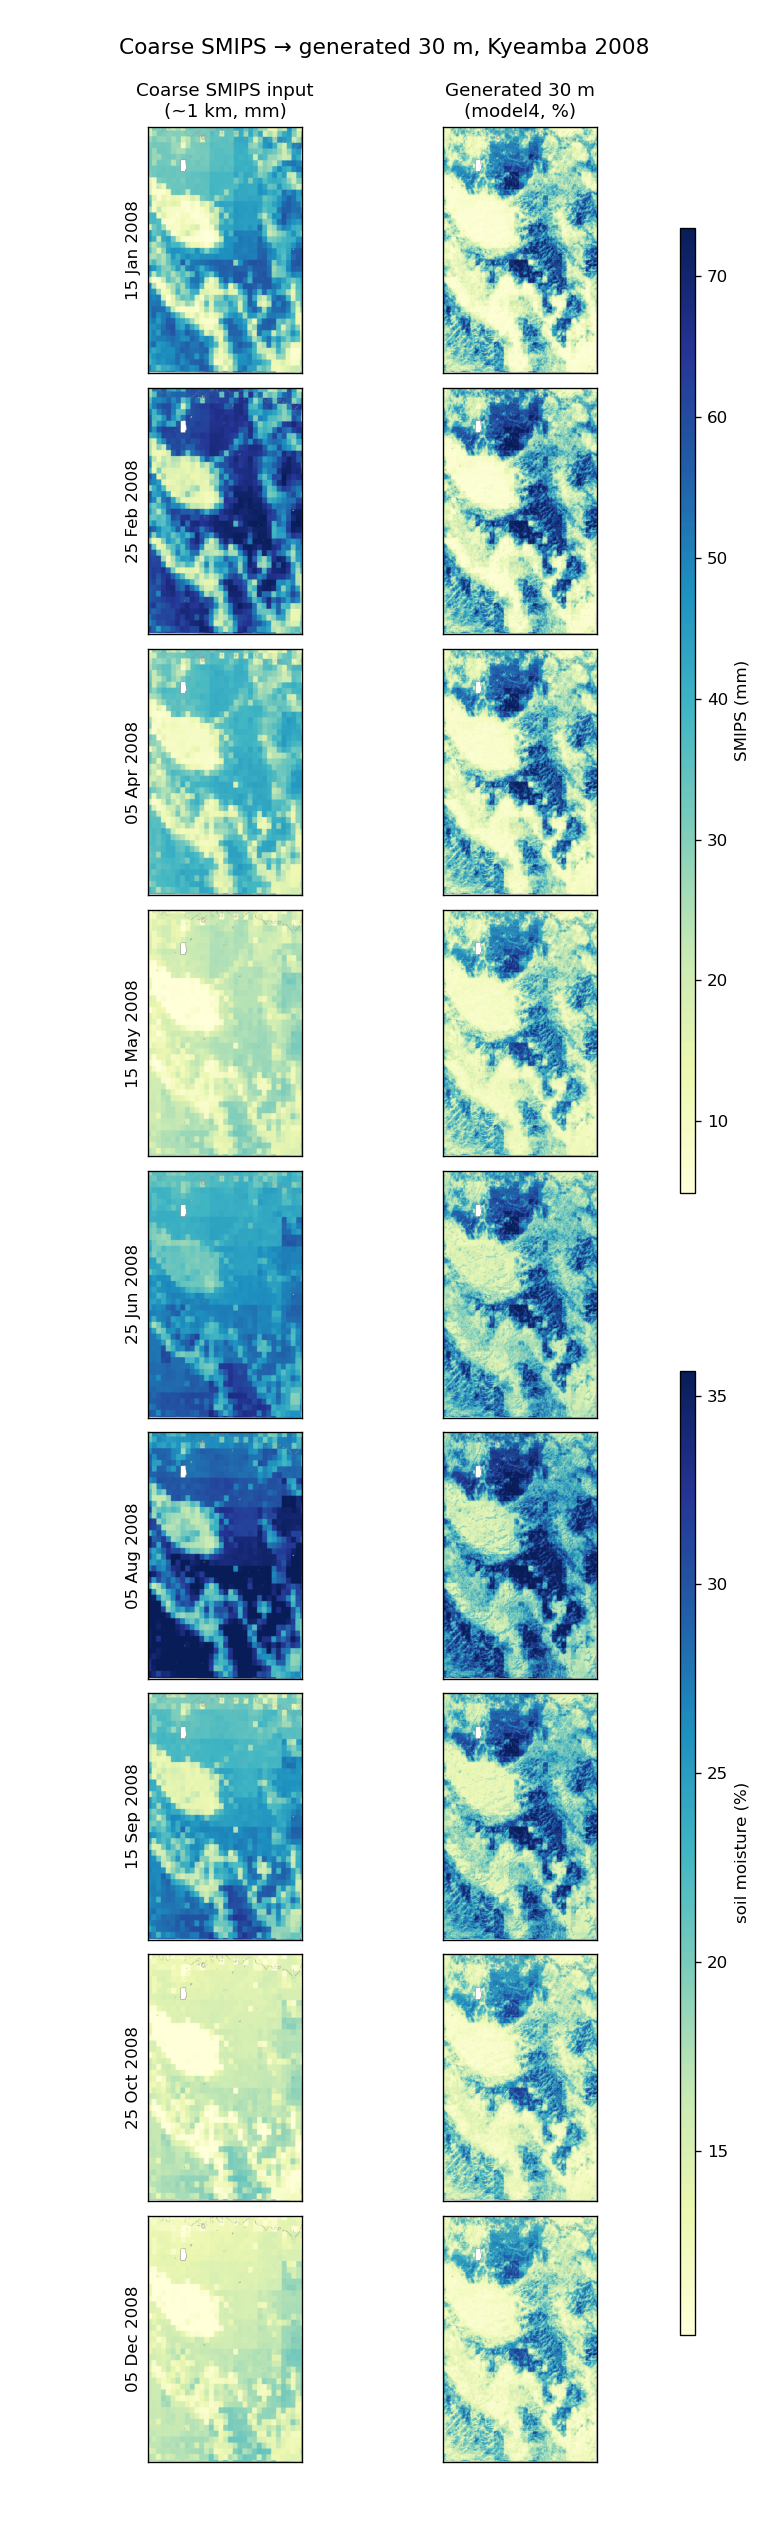
\includegraphics[width=\textwidth]{downscale_gallery_paired.png}
\caption{Coarse ${\approx}1$\,km SMIPS (left, mm) beside the generated 30\,m
field (right, \%), Kyeamba focus area, nine dates through 2008. Each row shows
the downscaling for one date; the sequence of rows shows the seasonal cycle.}
\label{fig:gallery}
\end{figure}

\begin{figure}[p]
\centering
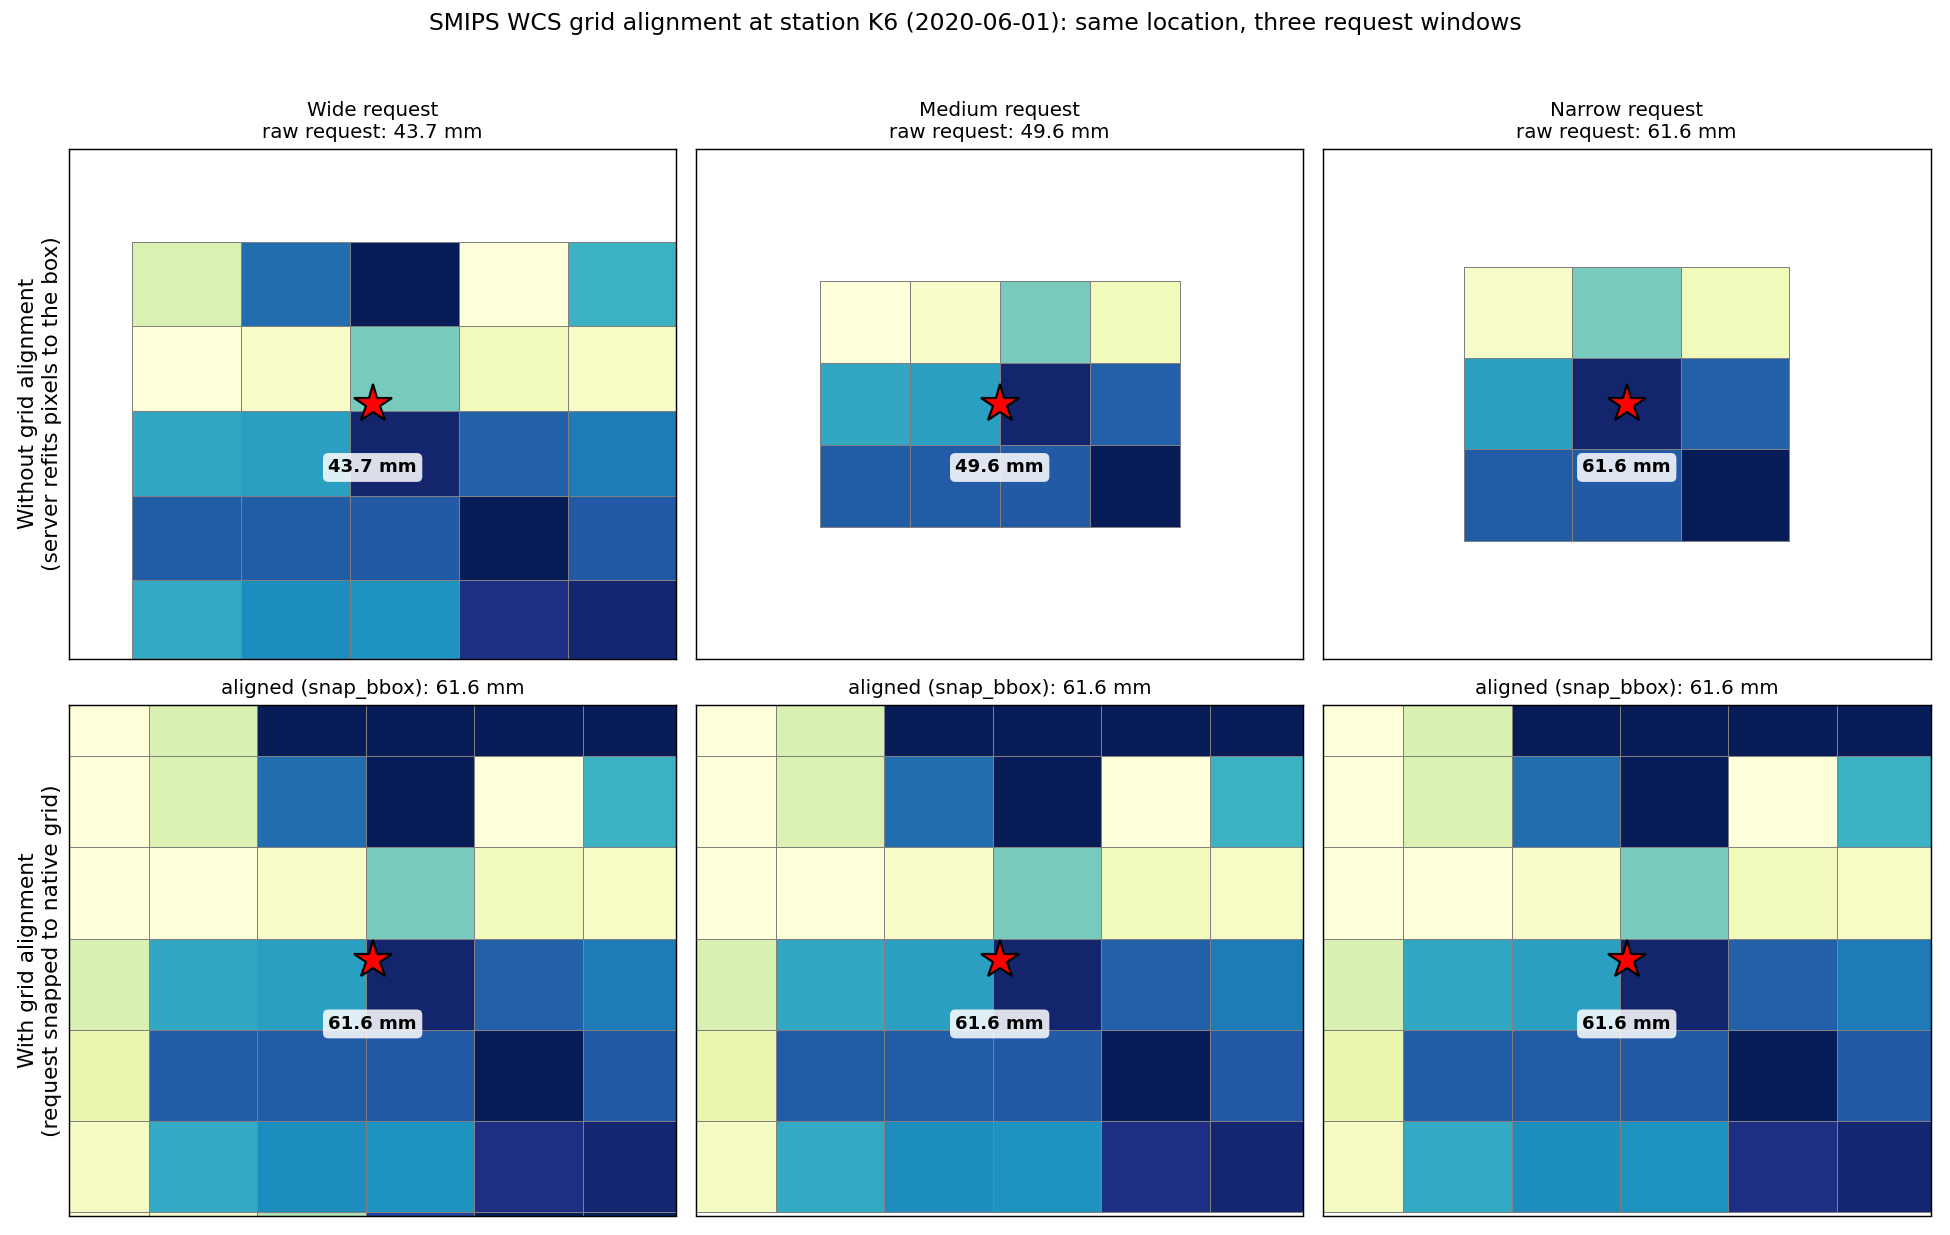
\includegraphics[width=\textwidth]{grid_alignment.png}
\caption{SMIPS retrieval: snapping requests to the native WCS grid removes the
dependence of sampled values on the request window.}
\label{fig:gridalign}
\end{figure}

\begin{figure}[p]
\centering
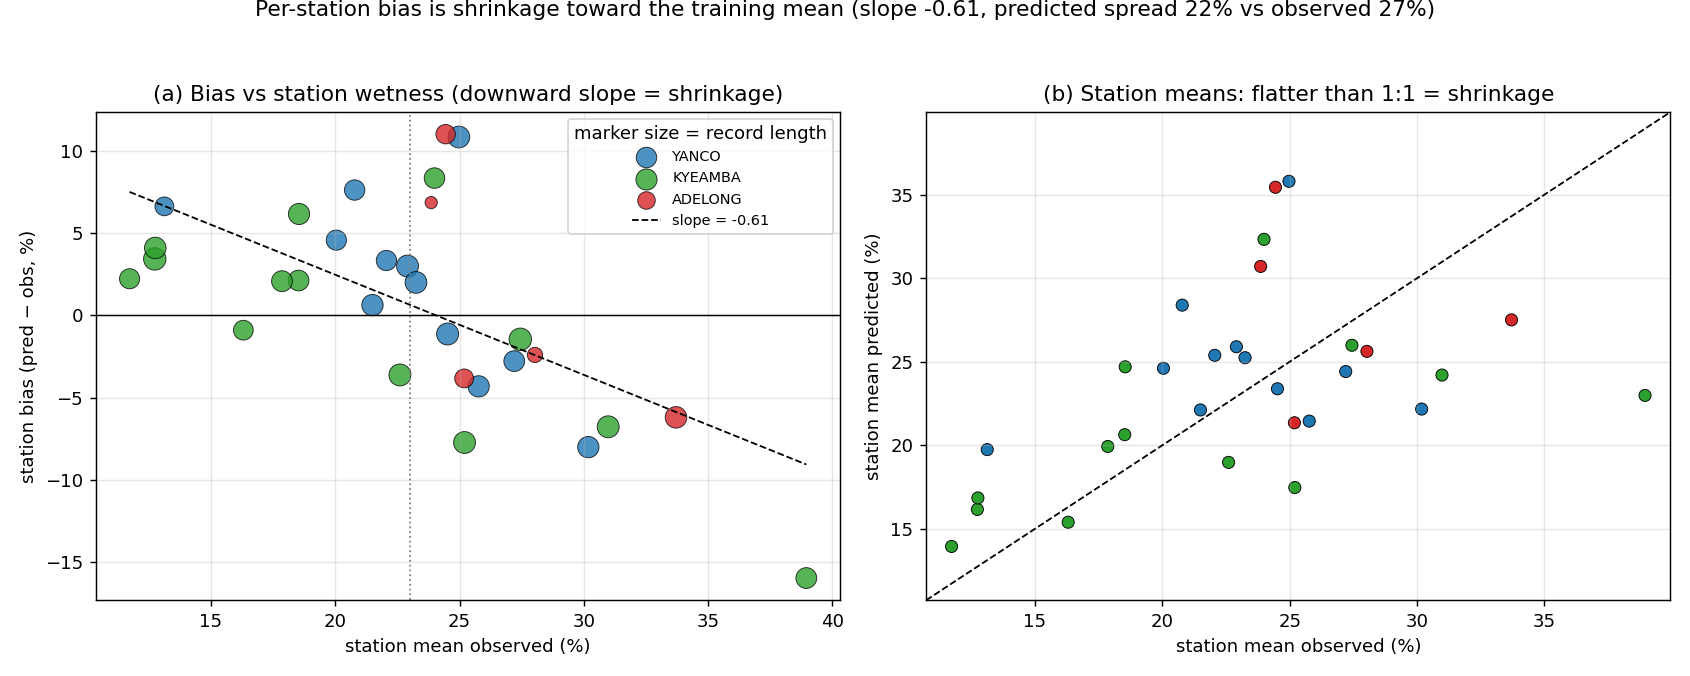
\includegraphics[width=\textwidth]{shrinkage_diagnostic.png}
\caption{The baseline failure mode (model~1): per-station bias is shrinkage
towards the training mean --- dry stations predicted too wet, wet stations too
dry.}
\label{fig:shrinkage}
\end{figure}

\begin{figure}[p]
\centering
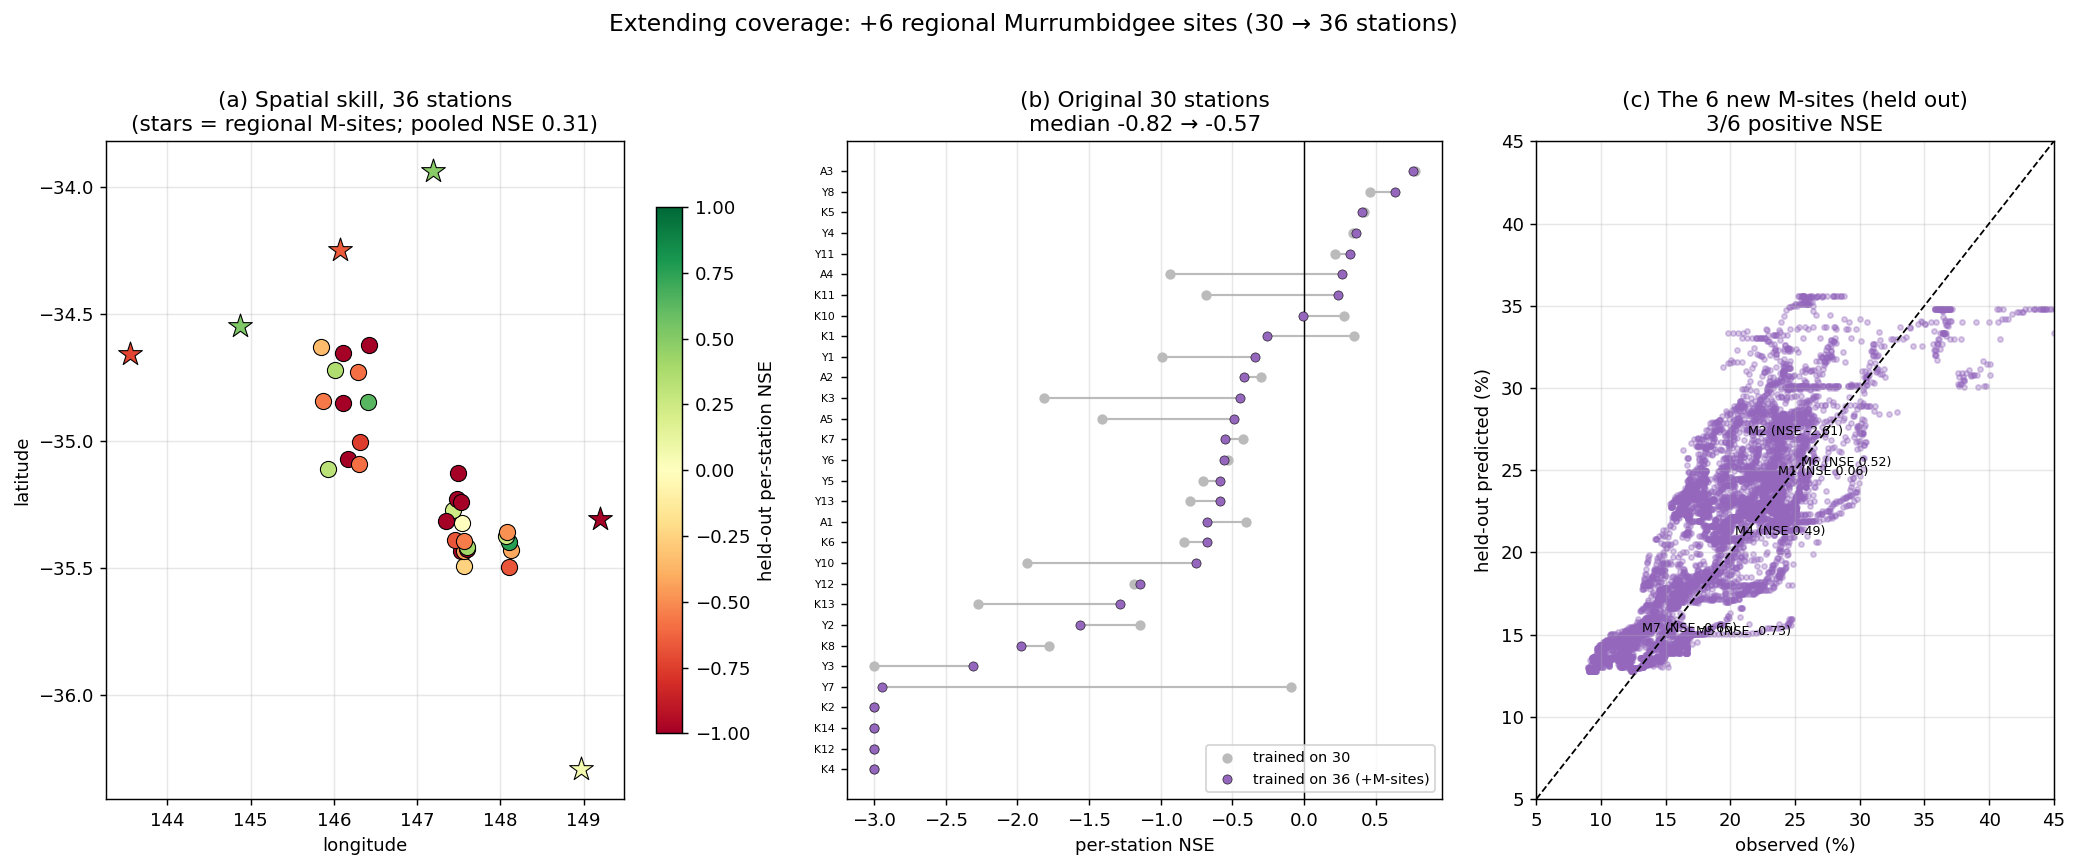
\includegraphics[width=\textwidth]{msites_extension.png}
\caption{The effect of spatial coverage: extending from 30 to 36 stations with
the regional M-sites drives model~1 negative ($-0.05$) while model~4 reaches
$+0.31$.}
\label{fig:msites}
\end{figure}

\begin{figure}[p]
\centering
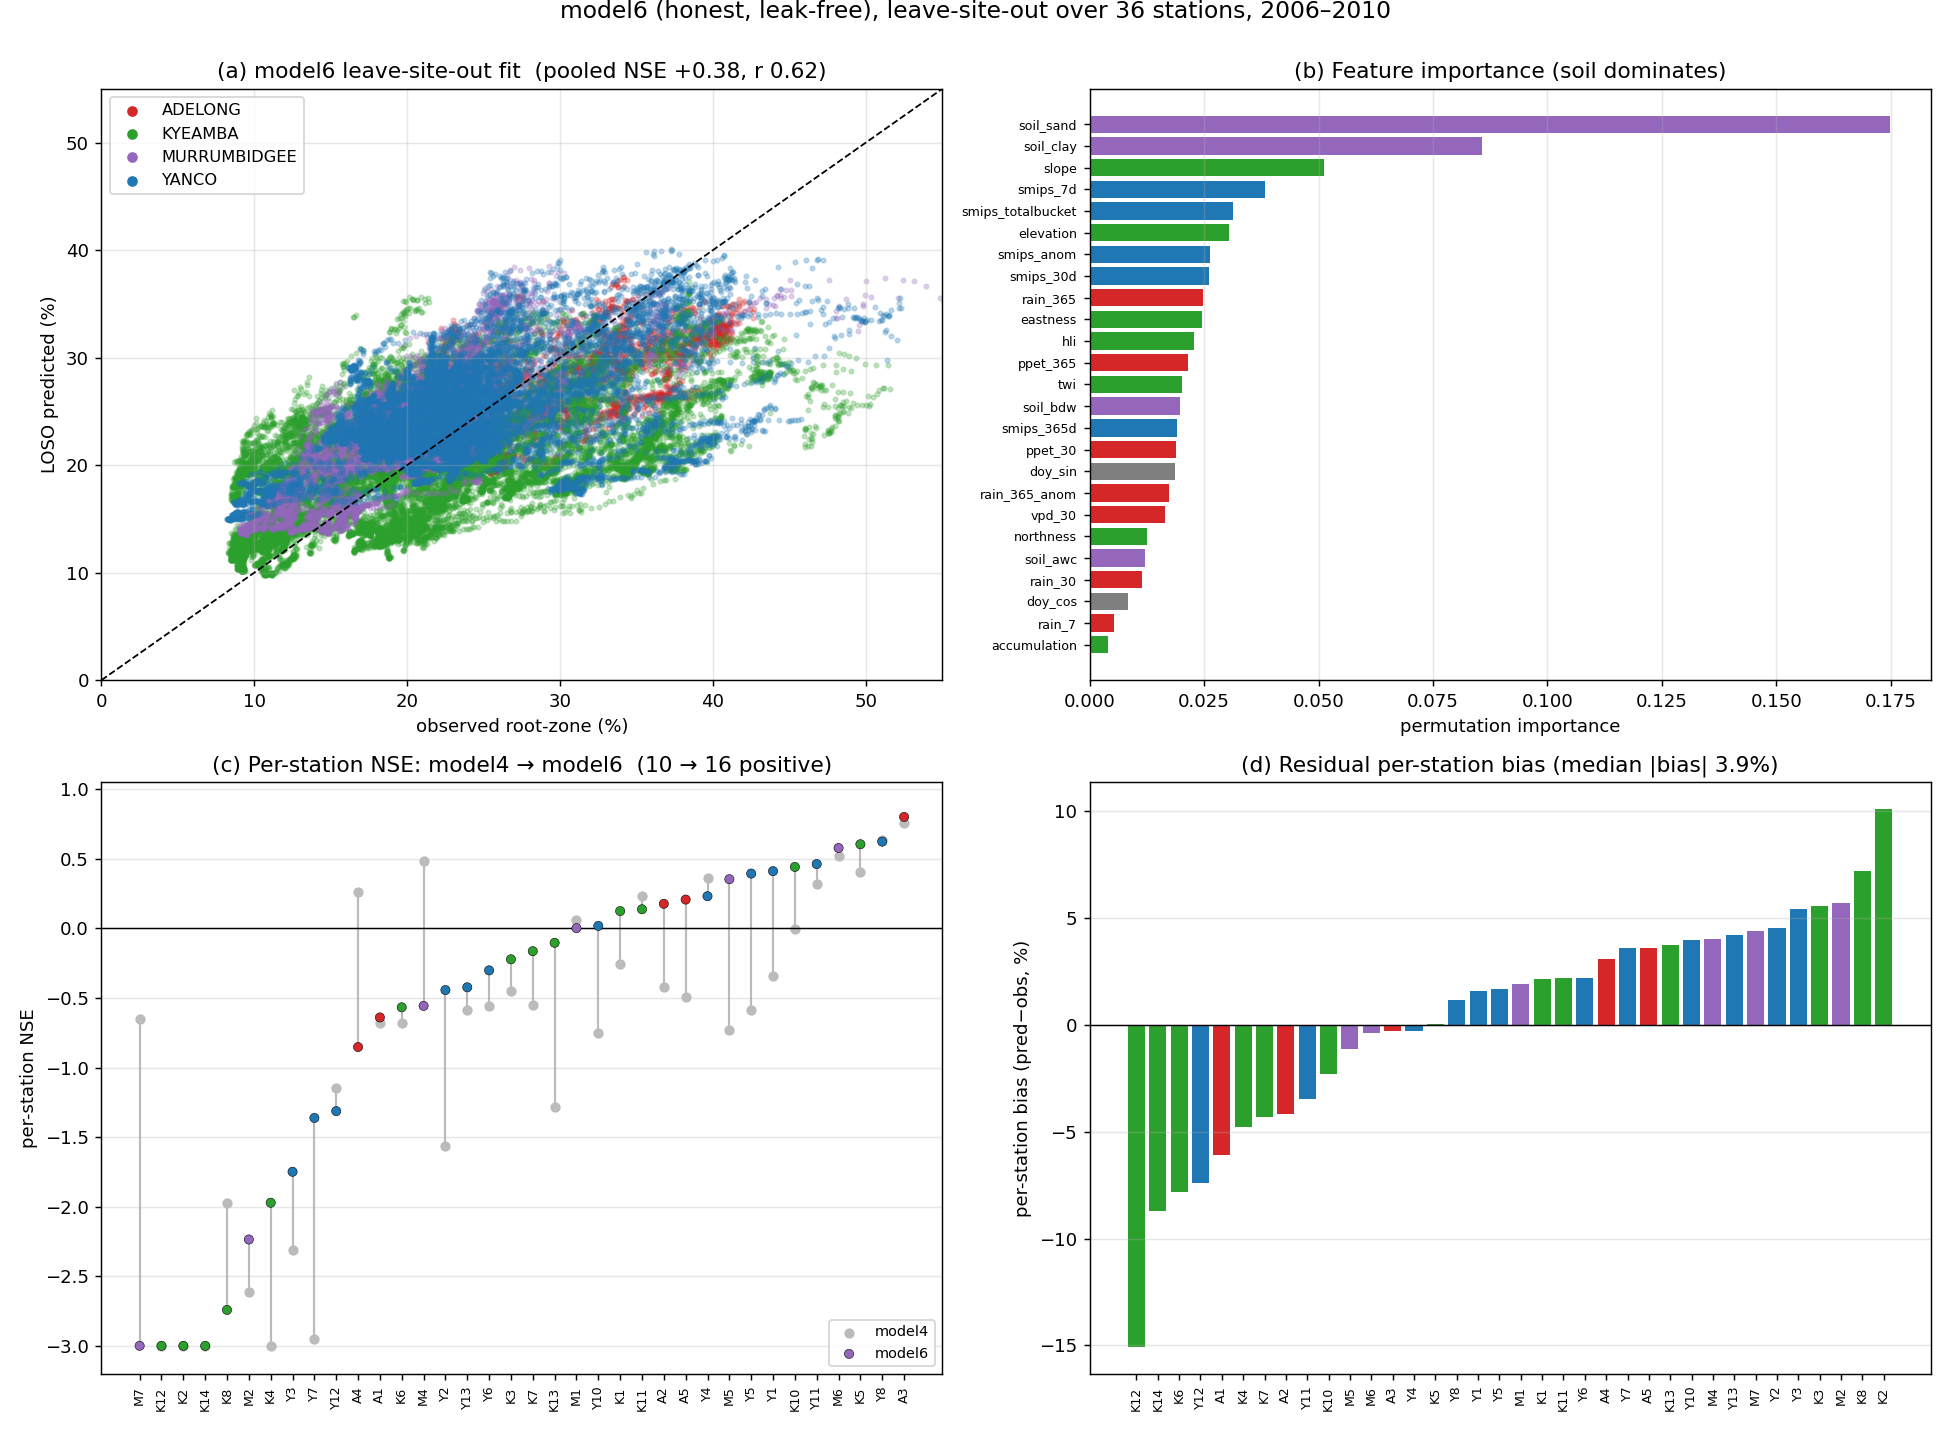
\includegraphics[width=\textwidth]{model6_results.png}
\caption{Model~6 leave-station-out results: fit, feature importance,
model~4 $\to$ 6 per-station NSE, and residual bias.}
\label{fig:m6results}
\end{figure}

\begin{figure}[p]
\centering
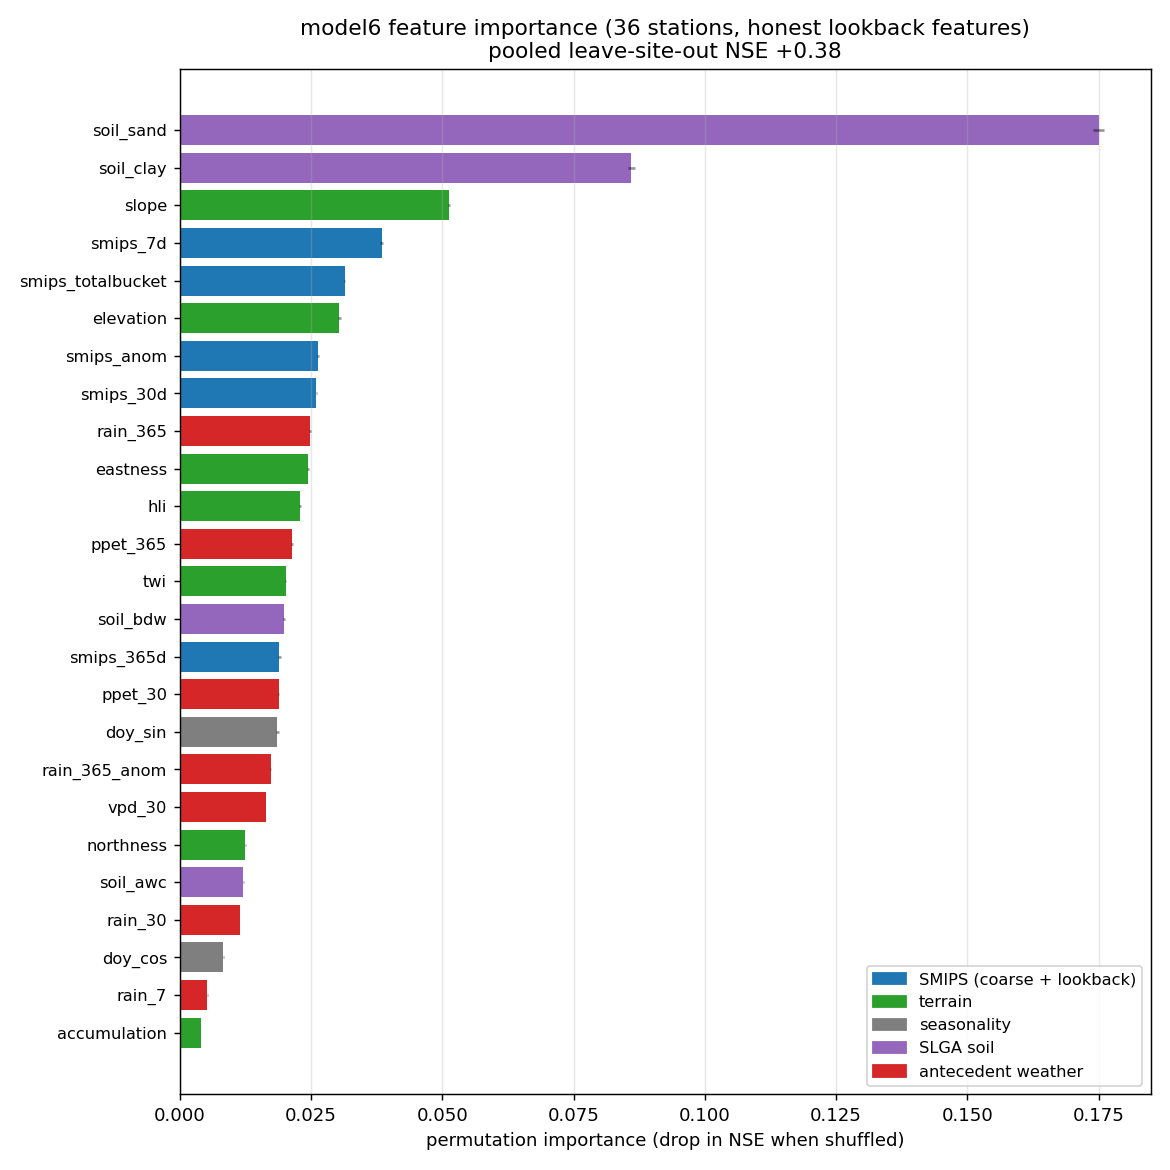
\includegraphics[width=0.85\textwidth]{model6_importance.png}
\caption{Model~6 permutation importance on the leak-free features: soil
texture leads, followed by terrain, the SMIPS lookback and the annual water
balance.}
\label{fig:m6importance}
\end{figure}

\begin{figure}[p]
\centering
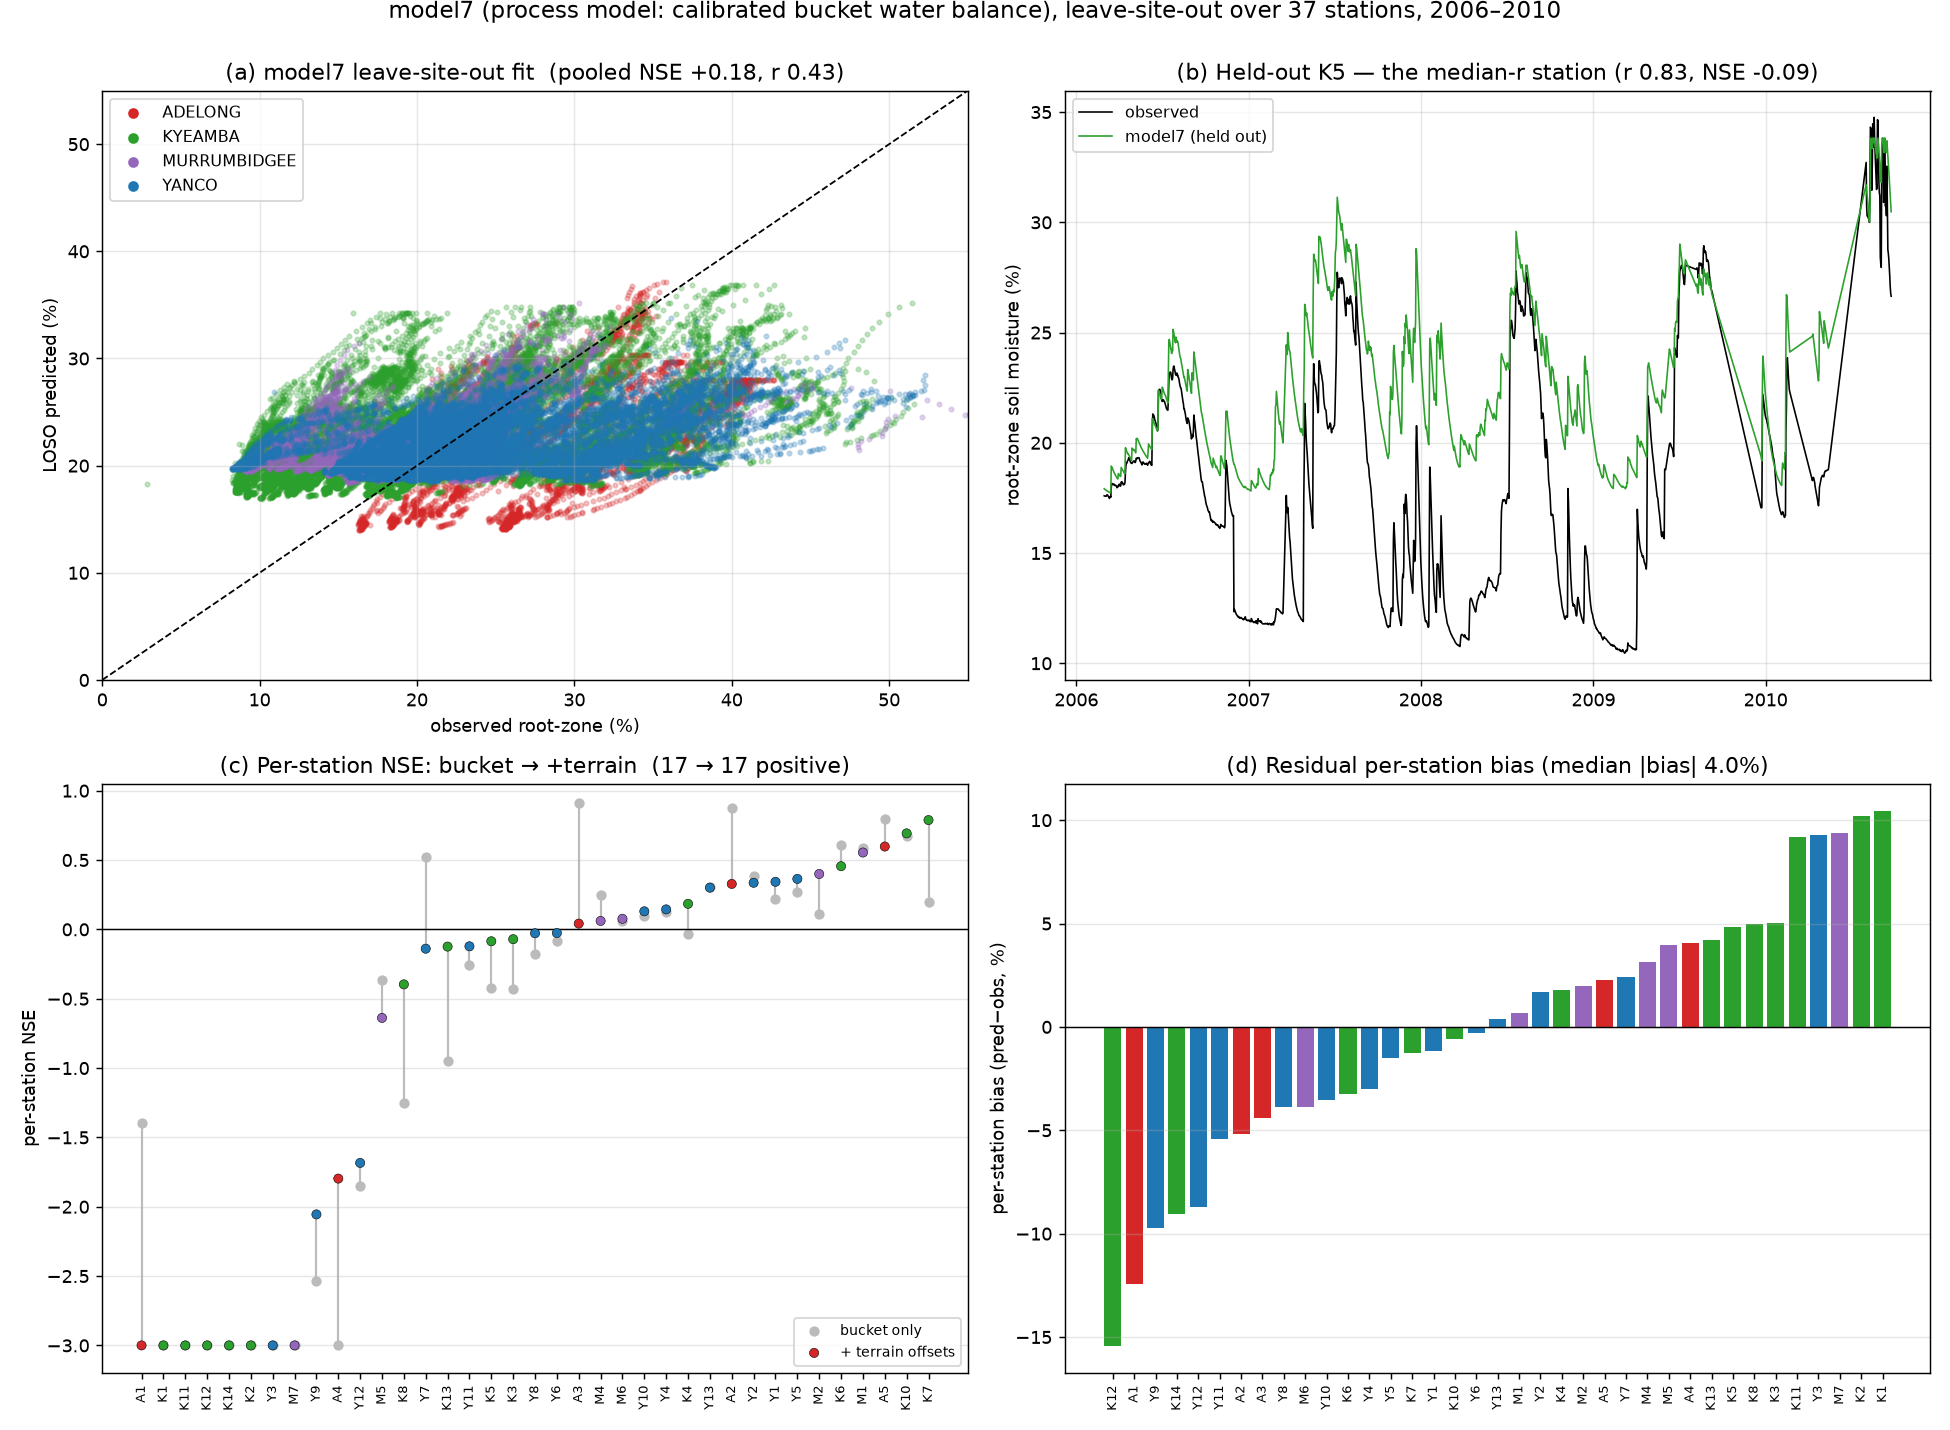
\includegraphics[width=\textwidth]{model7_results.png}
\caption{Model~7 (bucket water balance) leave-station-out results: the
predicted range compresses towards the middle (level shrinkage) while a
held-out station's dynamics are tracked through five years.}
\label{fig:m7results}
\end{figure}

\begin{figure}[p]
\centering
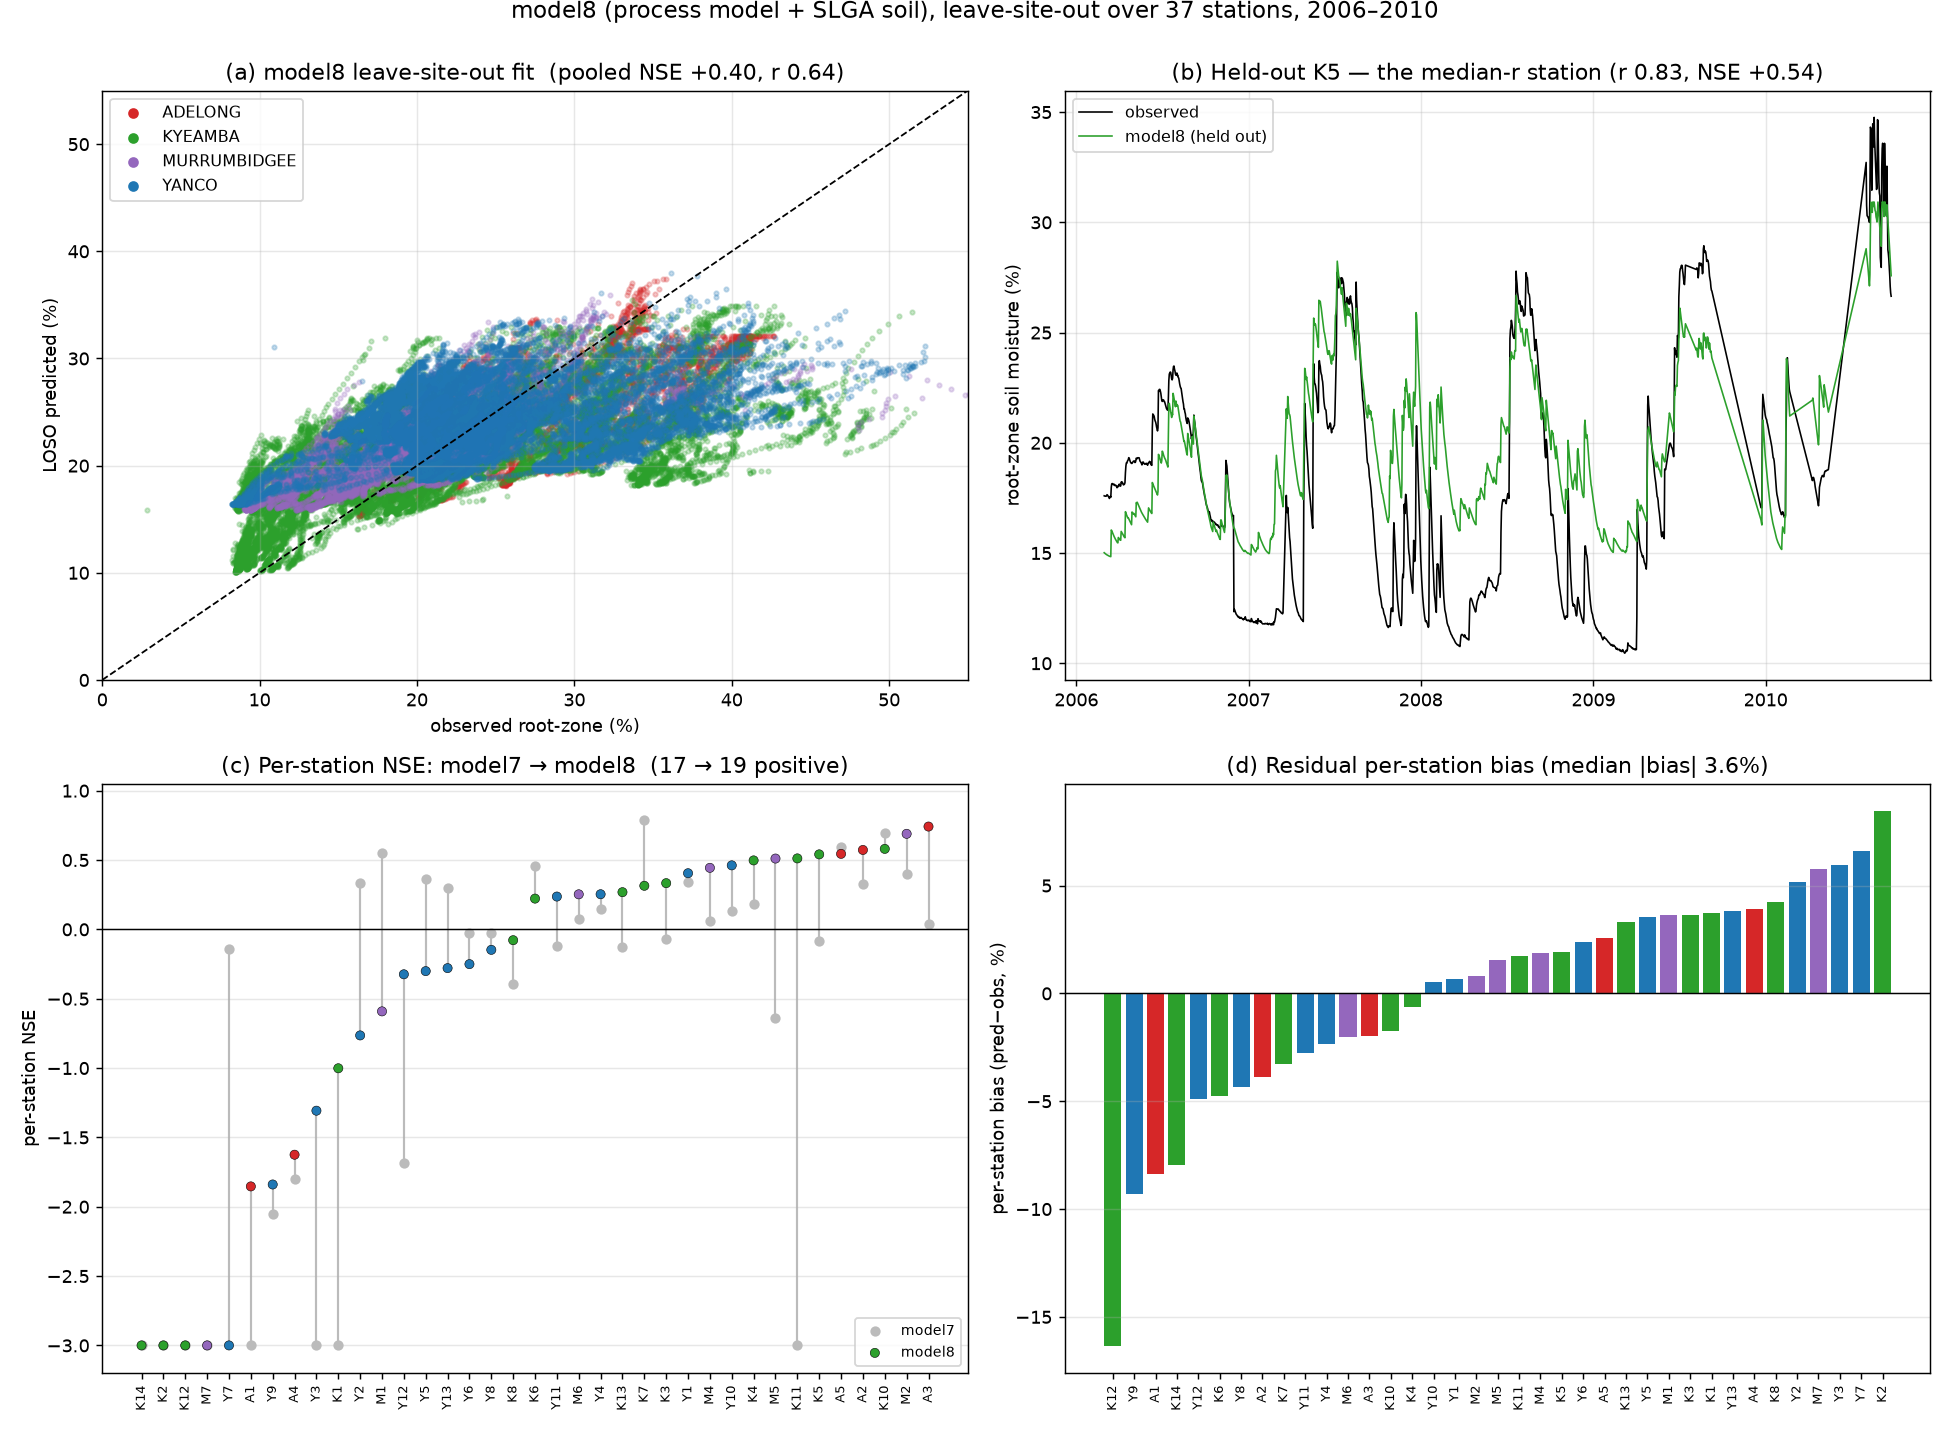
\includegraphics[width=\textwidth]{model8_results.png}
\caption{Model~8 leave-station-out results (pre-stack reference
configuration).}
\label{fig:m8results}
\end{figure}

\begin{figure}[p]
\centering
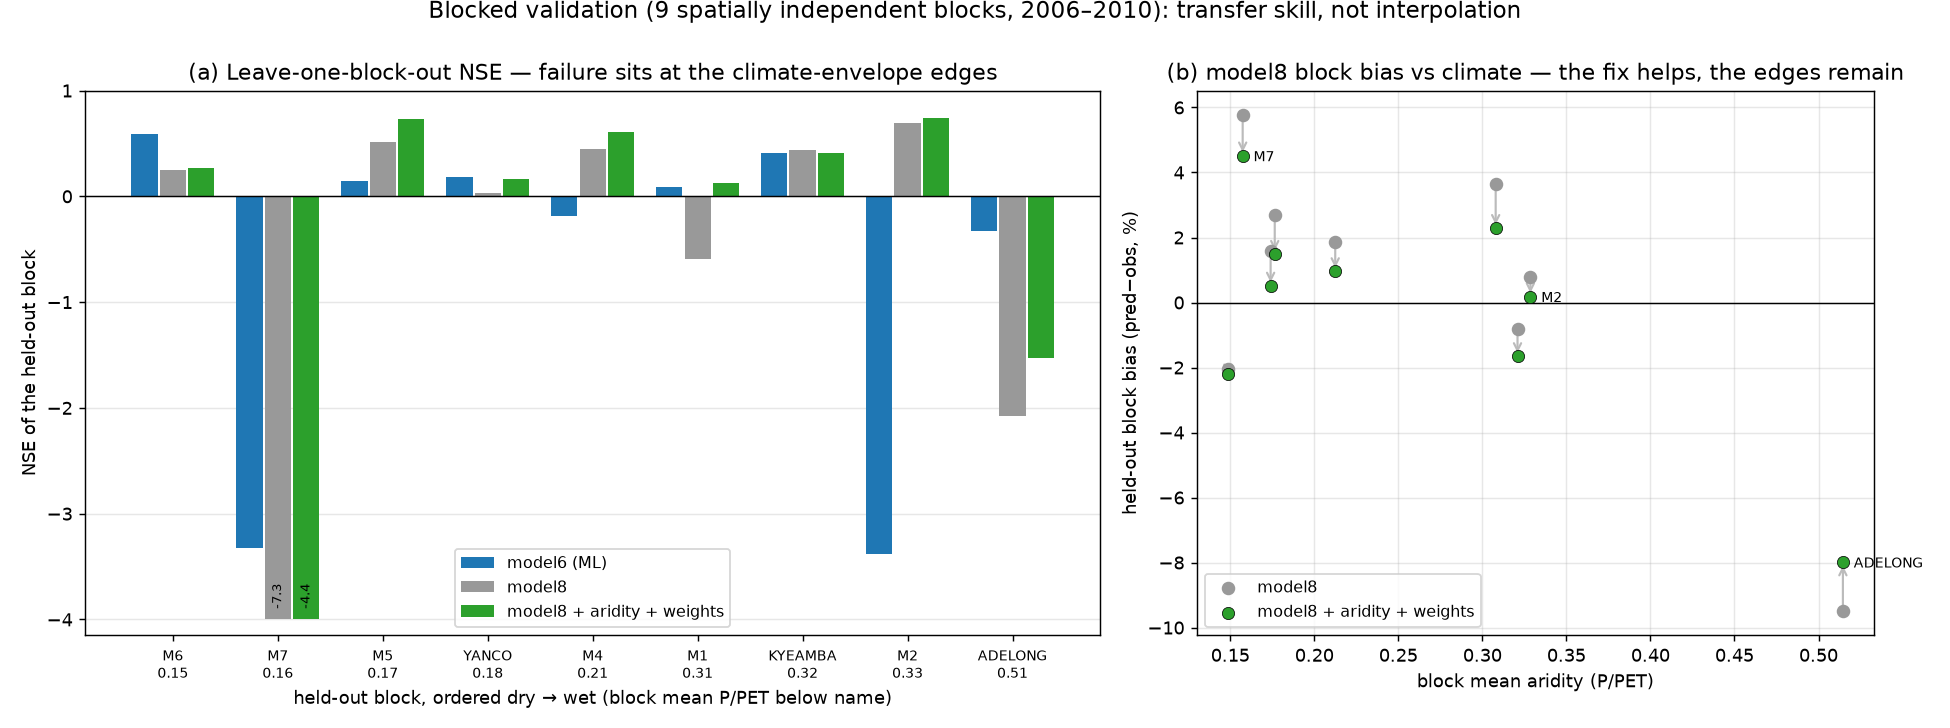
\includegraphics[width=\textwidth]{blocked_validation.png}
\caption{Blocked validation: the configuration ladder for models~8 and 6 under
leave-one-block-out over nine spatially independent districts.}
\label{fig:blocked}
\end{figure}

\begin{figure}[p]
\centering
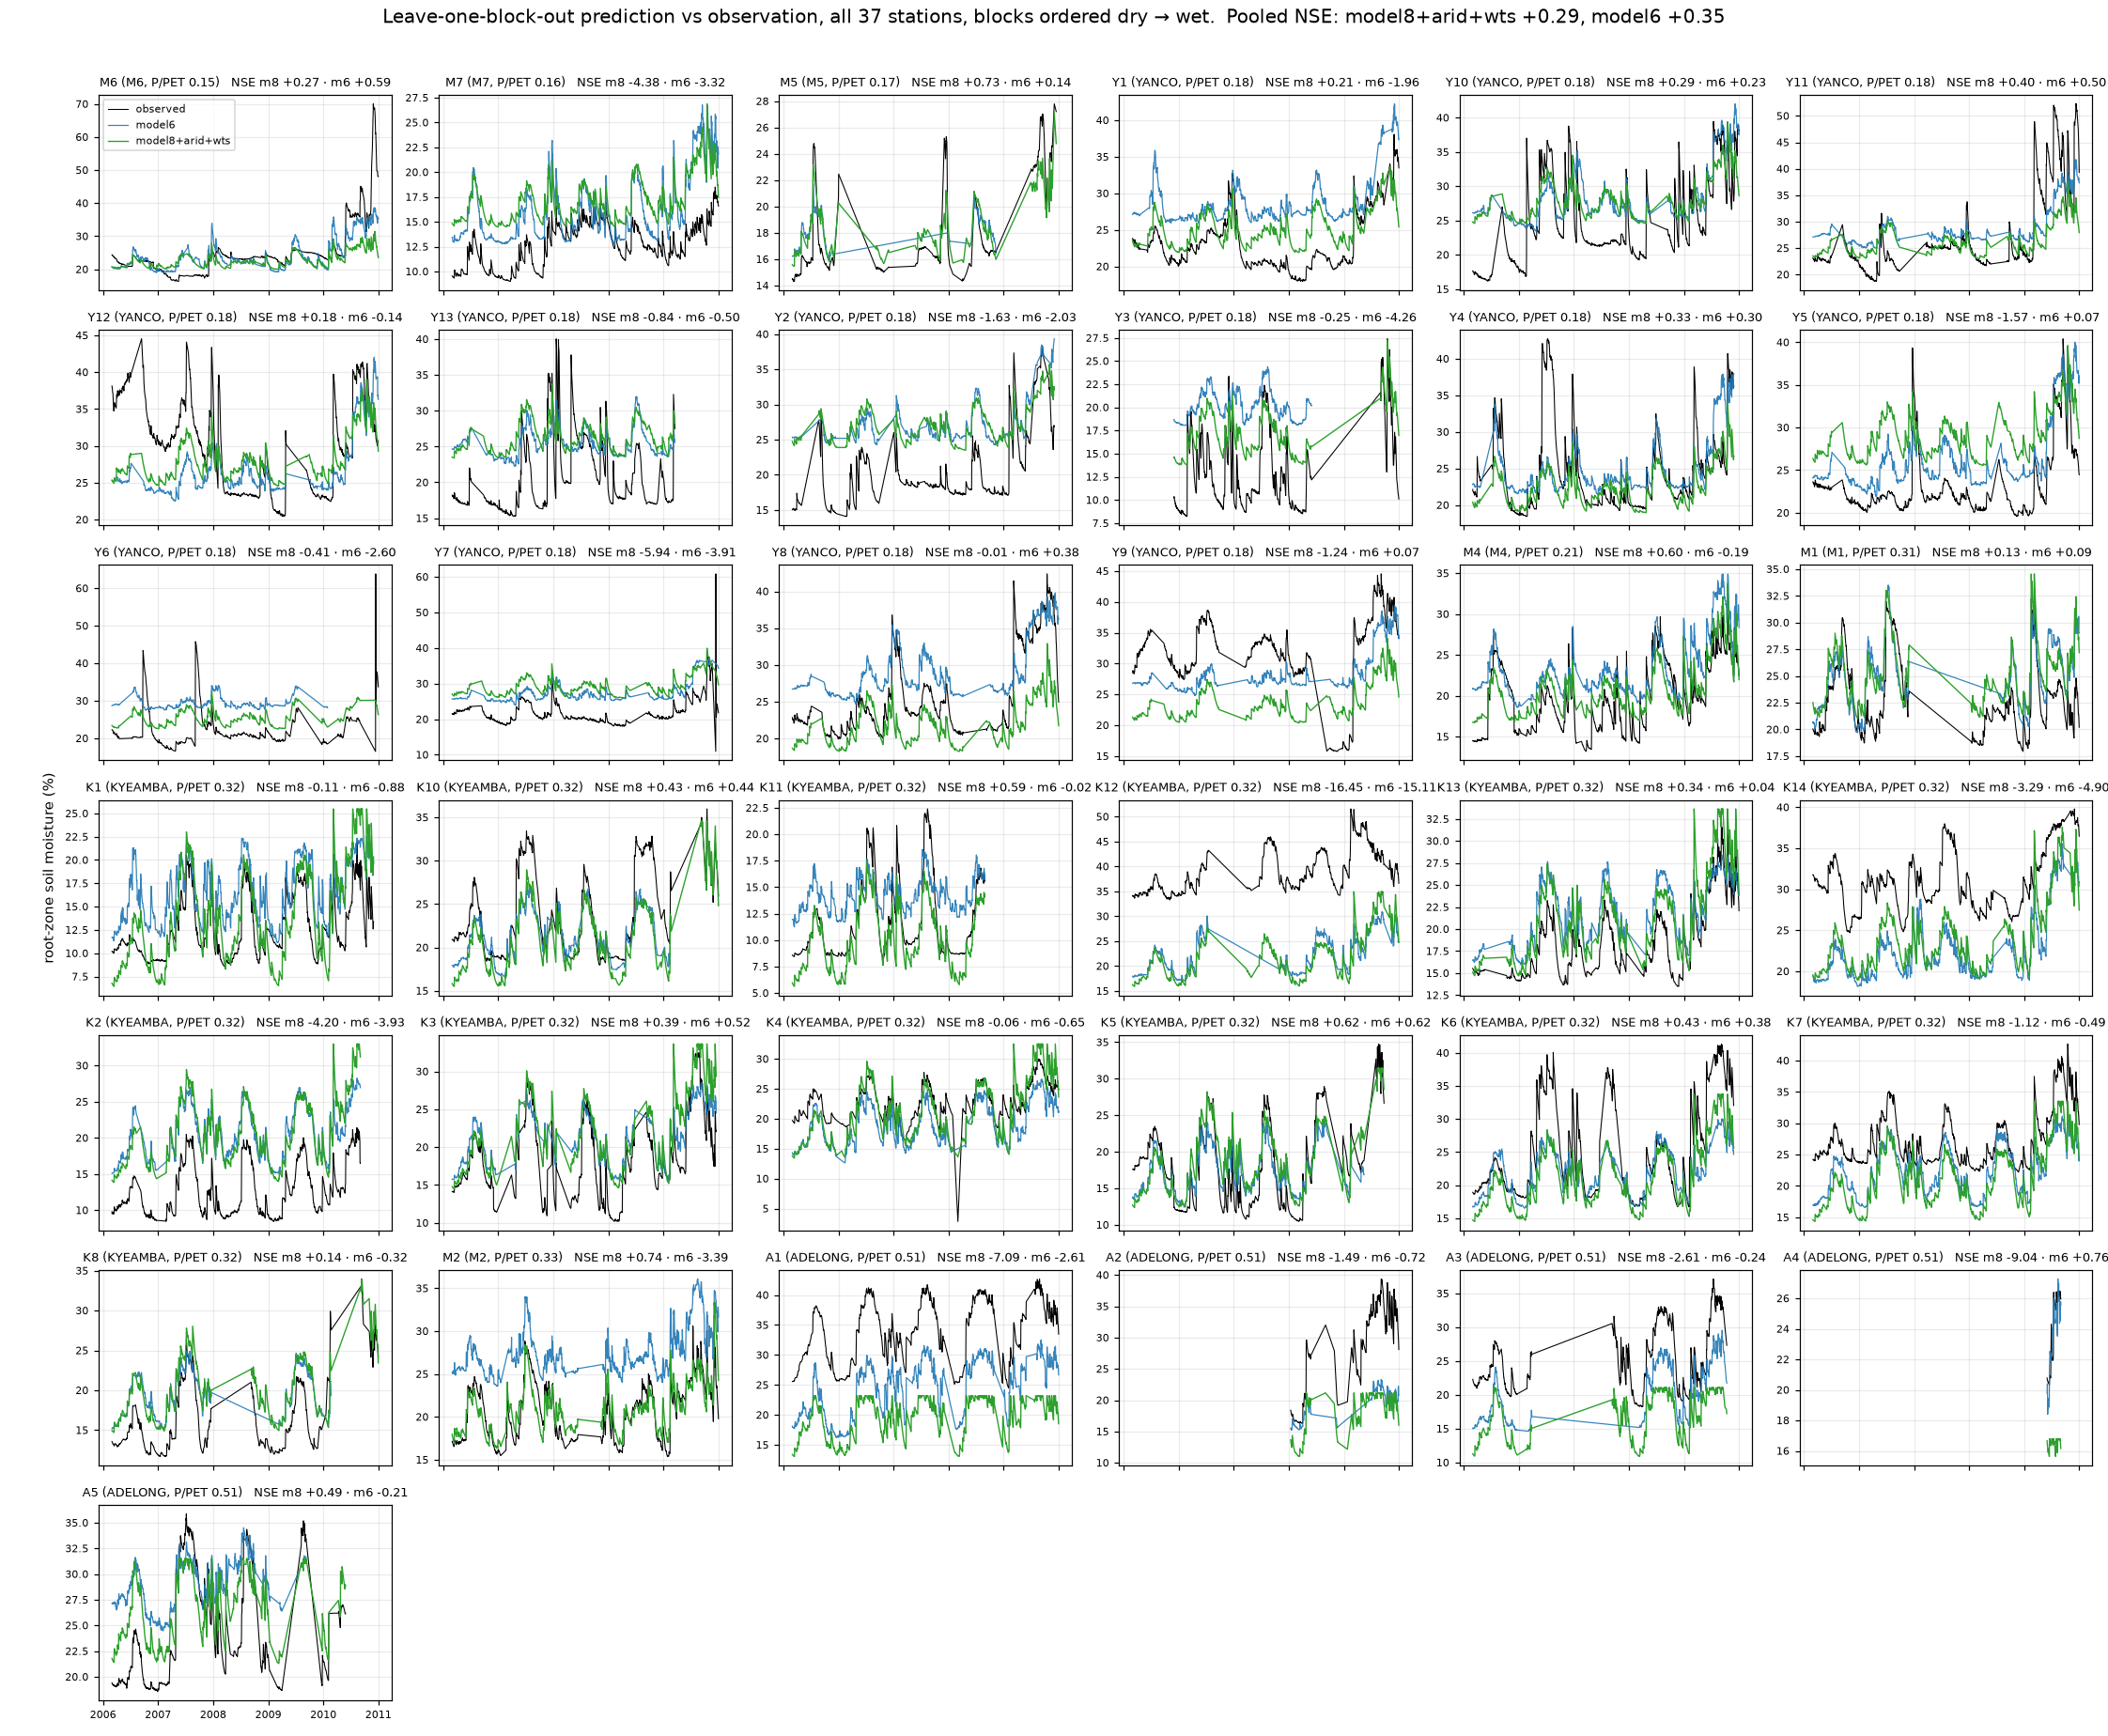
\includegraphics[width=\textwidth]{blocked_per_station.png}
\caption{Blocked hold-out, per-station series (observed in black; model~6
blue; final model~8 green), grouped by block from dry to wet. Both models
track the wetting--drying cycle; the errors manifest as whole-series
offsets.}
\label{fig:blockedstations}
\end{figure}

\begin{figure}[p]
\centering
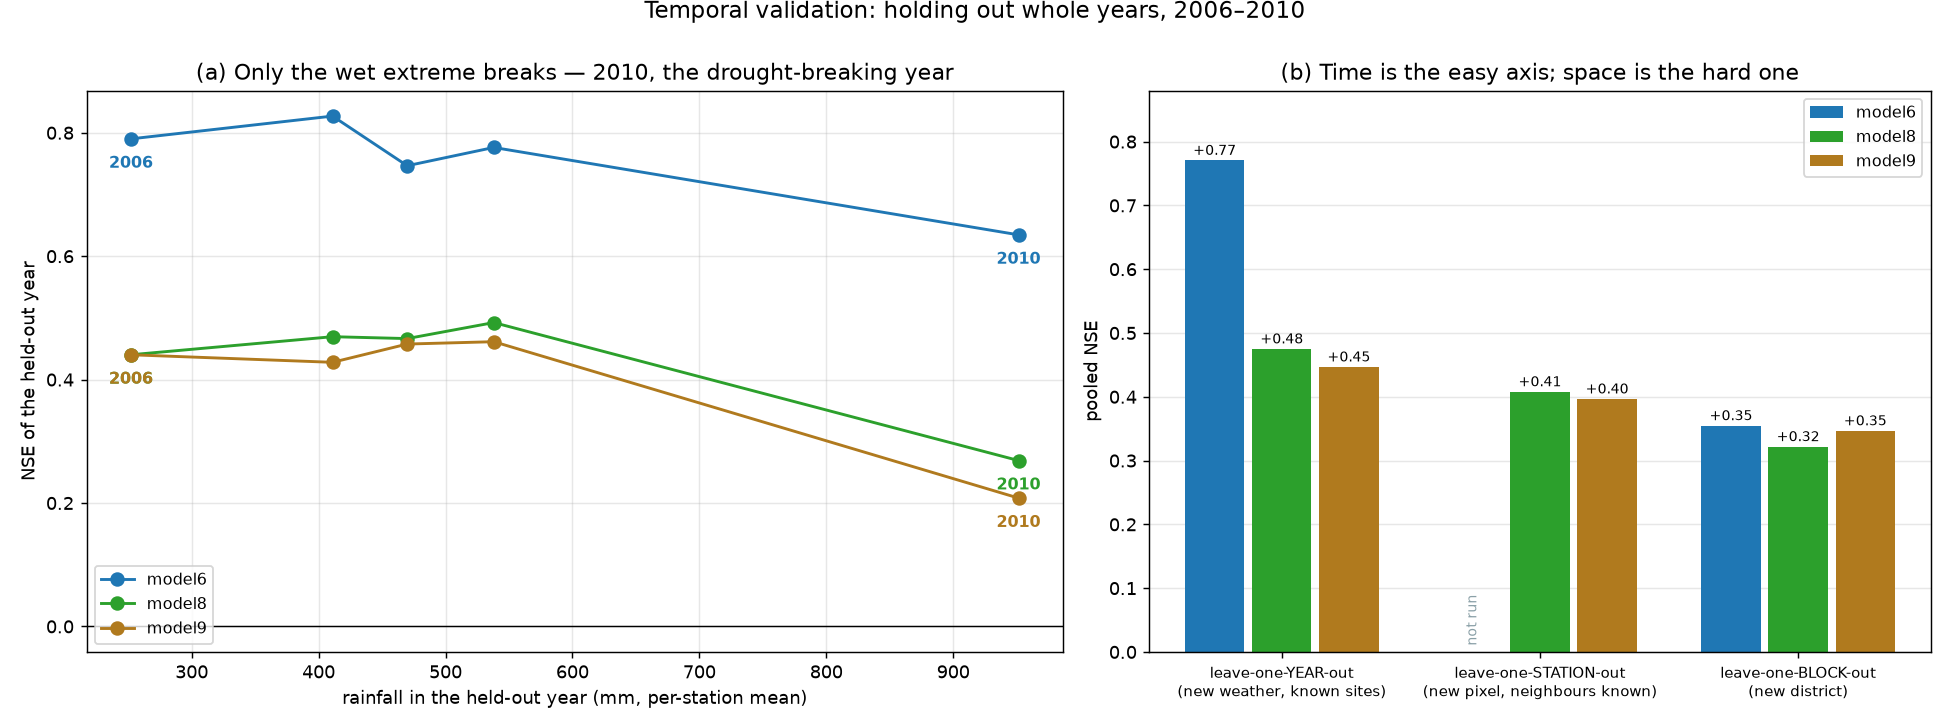
\includegraphics[width=\textwidth]{temporal_validation.png}
\caption{Temporal validation: leave-one-year-out across the drought break, and
the block\,$\times$\,year ladder.}
\label{fig:temporal}
\end{figure}

\begin{figure}[p]
\centering
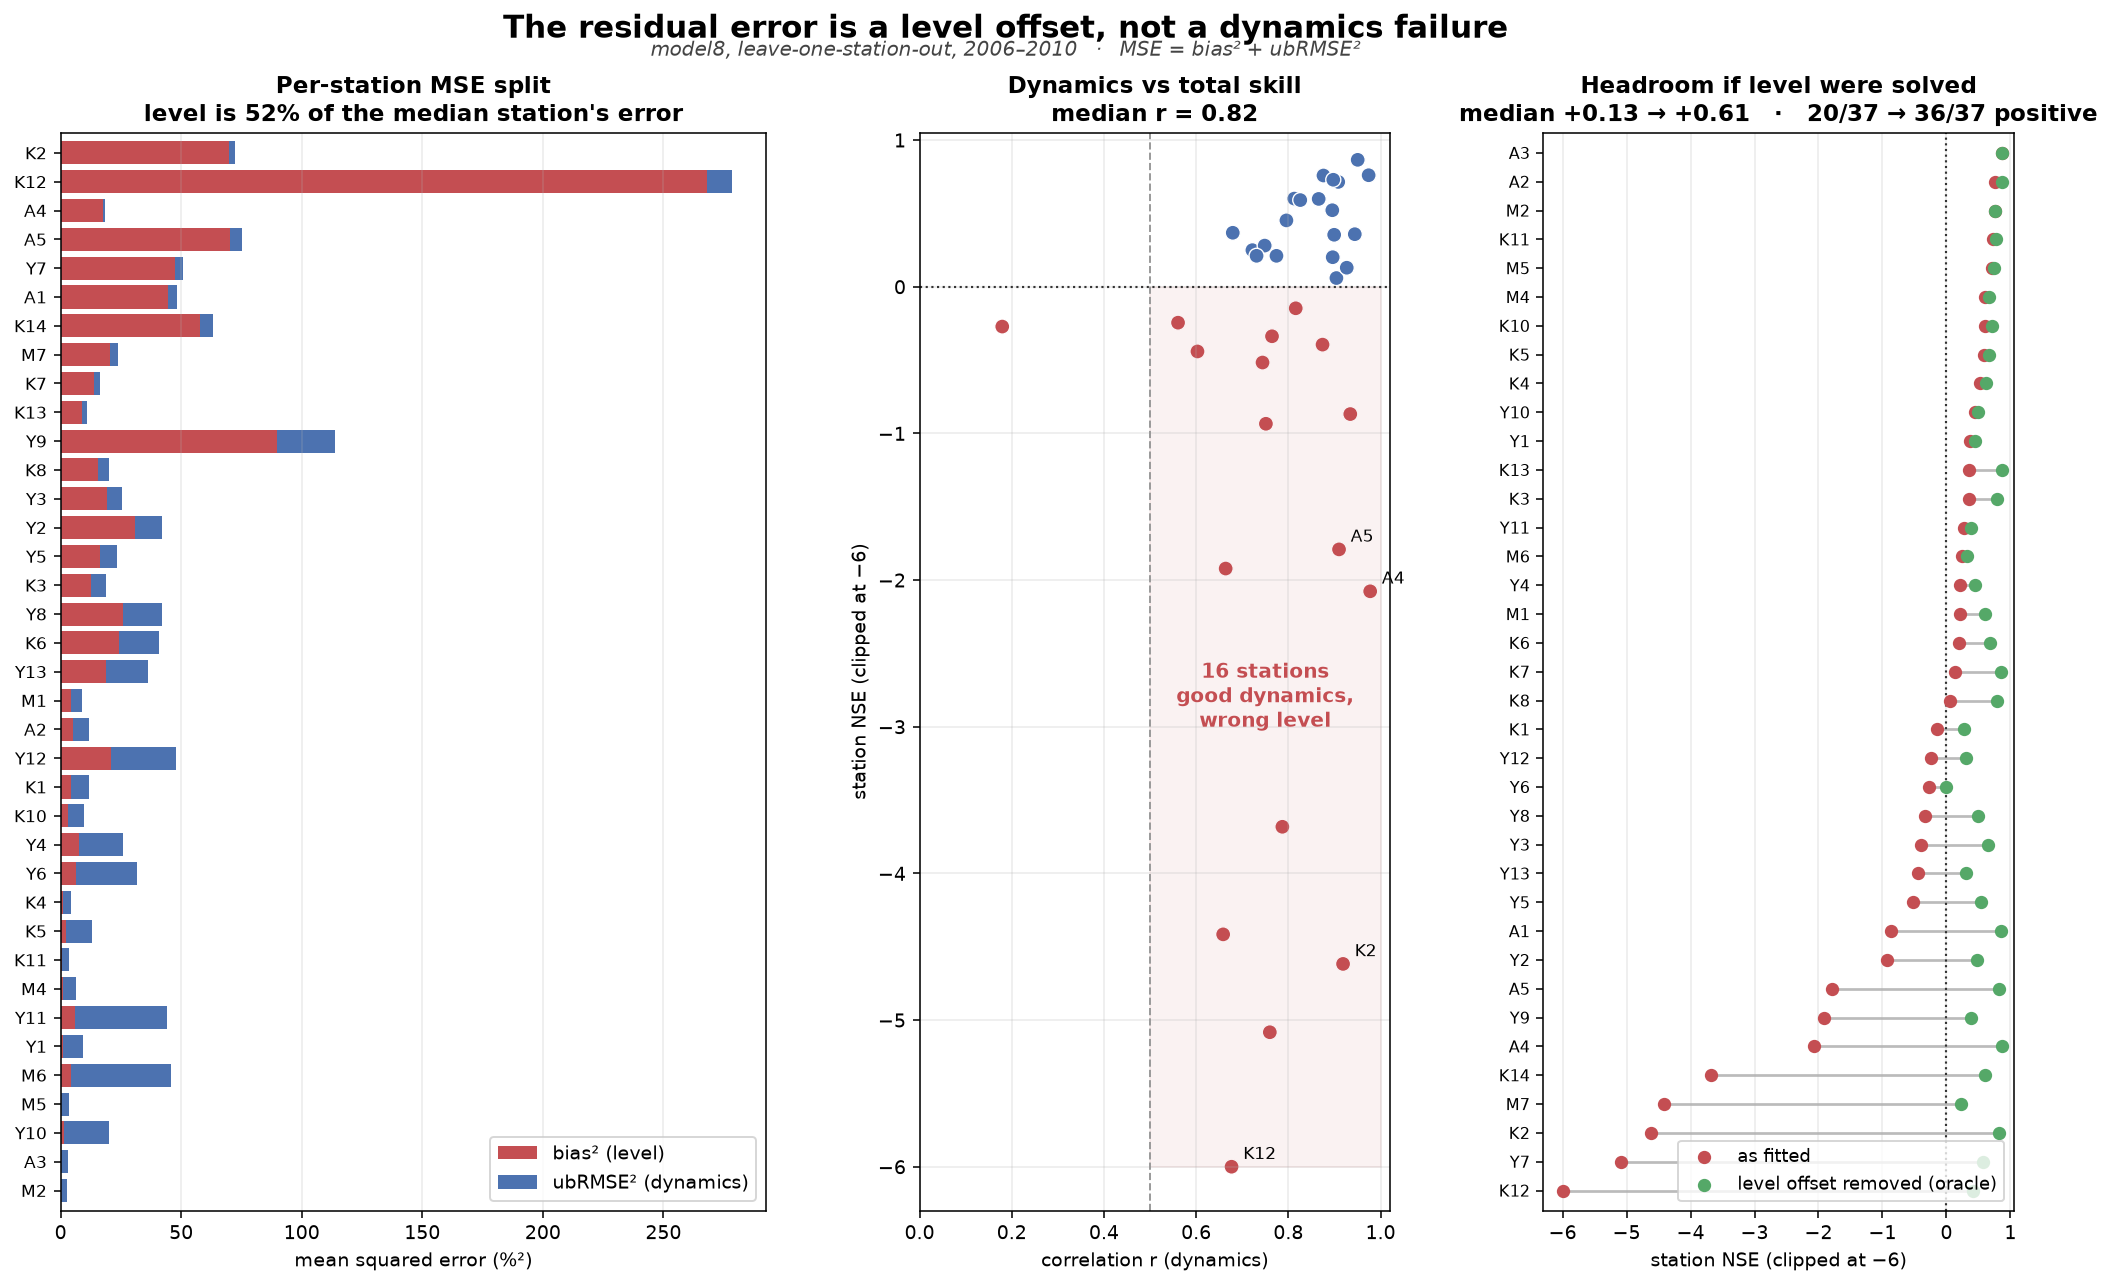
\includegraphics[width=\textwidth]{error_decomposition.png}
\caption{Error decomposition, $\mathrm{MSE} = \mathrm{bias}^2 + \ubrmse^2$,
per station: a median 52\,\% of held-out MSE is attributable to level, while
the dynamics are tracked at a median $r = 0.82$.}
\label{fig:decomp}
\end{figure}

\begin{figure}[p]
\centering
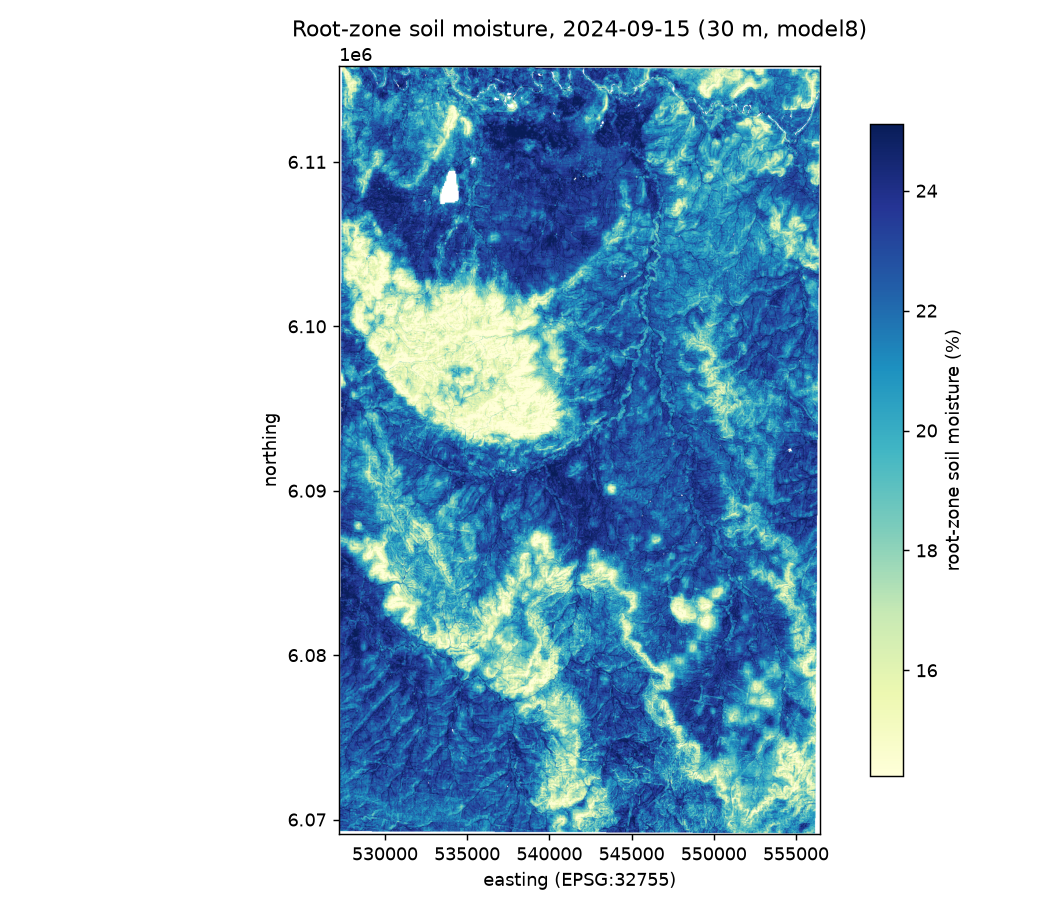
\includegraphics[width=\textwidth]{model8_predict_example.png}
\caption{The process model as a product: 30\,m field over Kyeamba for
2024-09-15, fourteen years after the training period and produced without
SMIPS. Drainage lines and valley floors are wet; ridges and steep blocks are
dry.}
\label{fig:m8map}
\end{figure}

\clearpage
\bibliographystyle{apalike}
\bibliography{references}

\end{document}
